\documentclass[12pt]{thesul}
%----------------------------------------------------------------------
%                               Packages
%----------------------------------------------------------------------
\usepackage[french]{babel}
\usepackage{acronym} % \ac[p], \acl[p], \acs[p], \acf[p]
\usepackage{biblatex}
\bibliography{biblio.bib}
\usepackage{booktabs} % \toprule, \midrule, \cmidrule, \bottomrule
\usepackage{caption}
\usepackage{csquotes}
\usepackage{hyperref}
\hypersetup{hidelinks}
\usepackage[inline]{enumitem}
\usepackage[french]{minitoc}

\usepackage{xcolor}
\AtBeginDocument{
\definecolor{pdfurlcolor}{rgb}{0,0,0}
\definecolor{pdfcitecolor}{rgb}{0,0,0}
\definecolor{pdflinkcolor}{rgb}{0,0,0}
\definecolor{light}{gray}{.85}
\definecolor{vlight}{gray}{.95}
\definecolor{darkgreen}{RGB}{77,172,38}
\definecolor{darkblue}{RGB}{5,113,176}
\definecolor{mydarkblue}{RGB}{116,173,209}
\definecolor{mydarkblueid}{RGB}{83,154,198}
\definecolor{mylightblue}{RGB}{171,217,233}
\definecolor{mydarkorange}{RGB}{244,109,67}
\definecolor{mylightorange}{RGB}{252,153,54}
\definecolor{mydarkred}{RGB}{215,48,39}
\definecolor{mydarkpurple}{RGB}{140,107,177}
\definecolor{mydarkpurpleid}{RGB}{136,86,167}
}

\usepackage{amssymb}
\usepackage{amsmath}
\interdisplaylinepenalty=2500
\newtheorem{definition}{Définition}
\newtheorem{myrule}{Règle}
\newtheorem{property}{Propriété}
\newtheorem{subproperty}{Propriété}[property]

\usepackage{algpseudocode}

\usepackage[draft,inline,nomargin,index]{fixme}
\fxsetup{theme=color,mode=multiuser,inlineface=\itshape,envface=\itshape}
\FXRegisterAuthor{go}{ago}{Gerald}
\FXRegisterAuthor{mn}{amn}{Matthieu}

\usepackage{tikz} % \begin{tikzpicture} \end{tikzpicture}
\usetikzlibrary{calc}
\usetikzlibrary{shapes.misc}

\usepackage[caption=false,font=footnotesize,labelfont=sf,textfont=sf]{subfig}

% Commands
%---------
\newcommand{\eg}{e.g. }
\newcommand{\ie}{c.-à-d. }

\newcommand{\headerparagraph}[1]{\textbf{\emph{#1}}\quad}

\newcommand{\inbb}[1]{\in \mathbb{#1}}
\newcommand{\mathlist}[2]{\set{#1_i \in #2}_{i \inbb{N}}}
\newcommand{\new}{\textbf{new}}
\newcommand{\trm}[1]{\mathit{#1}}
\newcommand{\set}[1]{\left\{#1\right\}} % set brace notation

\newcommand{\id}[3]{$\trm{#1}^{\trm{#2}}_{\trm{#3}}$}
\newcommand{\epoch}[1]{$\varepsilon_{#1}$}

\newcommand{\widthletter}{2em}
\newcommand{\widthblock}{3em}
\newcommand{\widthoriginepoch}{1.65em}
\newcommand{\widthepoch}{1.8em}

% Tikz styles
\tikzset{
    common/.style={anchor=west, draw, rectangle, minimum height=6mm},
    letter/.style={common, minimum width=\widthletter},
    block/.style={common, minimum width=\widthblock},
    epoch/.style={letter, rounded rectangle, rounded rectangle east arc=0pt, minimum width=\widthepoch},
    point/.style={insert path={ node[scale=5*sqrt(\pgflinewidth)]{.} }},
    op/.style={draw, circle, minimum size=2.7em},
    causalop/.style={op, double=white, inner sep=2pt},
    gc-rule-1/.style={dashed, thick, darkblue},
    gc-rule-2/.style={densely dotted, thick, darkgreen},
    cross/.style={
        path picture={
            \draw[mydarkred, very thick]
                (path picture bounding box.south east)--(path picture bounding box.north west)
                (path picture bounding box.south west)--(path picture bounding box.north east);
        }
    }
}


%-------------------------------------------------------------------
%                             Marges
%-------------------------------------------------------------------

% pour positionner les vraies marges:
%\SetRealMargins{1mm}{1mm}

%-------------------------------------------------------------------
%                             En-têtes
%-------------------------------------------------------------------

% Les en-têtes: quelques exemples
%\UppercaseHeadings
%\UnderlineHeadings
%\newcommand\bfheadings[1]{{\bf #1}}
%\FormatHeadingsWith{\bfheadings}
%\FormatHeadingsWith{\uppercase}
%\FormatHeadingsWith{\underline}
\newcommand\upun[1]{\uppercase{\underline{\underline{#1}}}}
\FormatHeadingsWith\upun

\newcommand\itheadings[1]{\textit{#1}}
\FormatHeadingsWith{\itheadings}

% pour avoir un trait sous l'en-tete:
\setlength{\HeadRuleWidth}{0.4pt}

%-------------------------------------------------------------------
%                         Les références
%-------------------------------------------------------------------

\NoChapterNumberInRef
\NoChapterPrefix

%-------------------------------------------------------------------
%                           Brouillons
%-------------------------------------------------------------------

% ceci ajoute une marque « brouillon » et la date
\ThesisDraft

%-------------------------------------------------------------------
%                   Pour collecter un glossaire et un index
%-------------------------------------------------------------------

\makeglossary
\makeindex

%-------------------------------------------------------------------
%                           Acronymes
%-------------------------------------------------------------------

% Acronyms
% --------
% \input{assets/acronyms.tex}
\acrodef{ADT}[ADT]{Abstract Data Type}
\acrodefplural{ADT}[ADTs]{Abstract Data Types}
\acrodef{CRDT}[CRDT]{Conflict-free Replicated Data Type}
\acrodefplural{CRDT}[CRDTs]{Conflict-free Replicated Data Types}
\acrodef{JIT}[JIT]{Just-In-Time}
\acrodef{LCA}[PPAC]{Plus Petit Ancêtre Commun}
\acrodef{OT}[OT]{Operational Transformation}
\acrodefplural{OT}[OT]{Operational Transformations}
\acrodef{P2P}[P2P]{Pair-à-Pair}
\acrodef{SEC}[SEC]{Cohérence forte à terme}

%-------------------------------------------------------------------
%                           Couleurs
%-------------------------------------------------------------------

% \input{assets/colours.tex}

%-------------------------------------------------------------------
%                     Global custom tikz commands
%-------------------------------------------------------------------

% \input{assets/tikz_presets.tex}

\begin{document}


      \OddHead={{\leftmark\rightmark}{\hfil\slshape\rightmark}}
      \EvenHead={{\leftmark}{{\slshape\leftmark}\hfil}}
      \OddFoot={\hfil\thepage}
      \EvenFoot={\thepage\hfil}
      \pagestyle{ThesisHeadingsII}


%-------------------------------------------------------------------
%                          Encadrements
%-------------------------------------------------------------------

% encadre les chapitres dans la table des matières:
% (ces commandes doivent figurer apres \begin{document}

\FrameChaptersInToc
%\FramePartsInToc


%-------------------------------------------------------------------
%            Réinitialisation de la numérotation des chapitres
%-------------------------------------------------------------------

% Si la commande suivante est présente,
% elle doit figurer APRÈS \begin{document}
% et avant la première commande \part
\ResetChaptersAtParts

%-------------------------------------------------------------------
%               mini-tables des matières par chapitre
%-------------------------------------------------------------------

% préparer les mini-tables des matières par chapitre.
% (commande de minitoc.sty)
\dominitoc

%-------------------------------------------------------------------
%                         Page de titre:
%-------------------------------------------------------------------

\ThesisTitle{Ré-identification efficace dans les types de données répliquées sans conflit (CRDTs)}
\ThesisDate{TODO: Définir une date}
\ThesisAuthor{Matthieu Nicolas}

% Type de la these
\ThesisUL
% Jury:

% (ne pas mettre de \\ apres la dernière entree)

% Exemple de création d'une nouvelle catégorie dans le jury:

\NewJuryCategory{family}{\it Membre de la famille :}
                        {\it Membres de la famille :}

\family={Mon frère\\Ma sœur}

\def\blanc{\hspace*{1cm}}

\President    = {Stephan Merz}
\Rapporteurs  = {Le rapporteur 1&de Paris\\
                 Le rapporteur 2\\
                 \blanc suite&taratata\\
                 Le rapporteur 3}
\Examinateurs = {L'examinateur 1&d'ici\\
                 L'examinateur 2}
%\Invites=       {}

% Création de la page de titre:
\MakeThesisTitlePage

%-------------------------------------------------------------------


%-------------------------------------------------------------------
%                          remerciements
%-------------------------------------------------------------------

%\DontFrameThisInToc
\begin{ThesisAcknowledgments}
Les remerciements.
\end{ThesisAcknowledgments}

%-------------------------------------------------------------------
%                            dédicace
%-------------------------------------------------------------------

\begin{ThesisDedication}
Je dédie cette thèse\\
à ma machine.\\
Oui, à Pandore,\\
qui fut la première de toutes.
\end{ThesisDedication}


%-------------------------------------------------------------------
%                  écriture de `Chapitre' et `Partie'
%                      dans la table des matières
%-------------------------------------------------------------------

\WritePartLabelInToc
\WriteChapterLabelInToc

%-------------------------------------------------------------------
%                        table des matières
%-------------------------------------------------------------------

\tableofcontents

%-------------------------------------------------------------------
%              Exemple d'utilisation de \SpecialSection
%-------------------------------------------------------------------
%\SpecialSection{Introduction générale}

\DontWriteThisInToc
\listoffigures

\mainmatter
\NumberThisInToc
\chapter*{Introduction}
\minitoc
\section{Contexte}
\section{Questions de recherche}
\section{Contributions}
\section{Plan du manuscrit}
% Dans ce chapitre, nous revenons sur les contributions présentées dans cette thèse.
Nous rappelons le contexte dans lequel elles s'inscrivent, récapitulons leurs spécificités et apports, et finalement précisons plusieurs de leurs limites.
Puis, nous concluons ce manuscrit en présentant plusieurs pistes de recherche qui nous restent à explorer à l'issue de cette thèse.
La première s'inscrit dans la continuité directe de nos travaux sur un mécanisme de ré-identification pour \acp{CRDT} pour le type Séquence pour les applications \acf{LFS}.
Les dernières traduisent quant à elles notre volonté de recentrer nos travaux sur le domaine plus général des \acp{CRDT}.


% \NumberThisInToc
% \chapter*{Problématique}
% \minitoc
% \input{assets/chapter_problematic}

\NumberThisInToc
\chapter{État de l'art}
\minitoc

\begin{itemize}
  \item Contexte des systèmes distribués à large échelle
  \item Réplique les données afin de pouvoir supporter les pannes
  \item Adopte le paradigme de la réplication optimiste \cite{10.1145/1057977.1057980}
  \item Autorise les noeuds à consulter et à modifier la donnée sans aucune coordination entre eux
  \item Autorise alors les noeuds à diverger temporairement
  \item Permet d'être toujours disponible, de toujours répondre aux requêtes même en cas de partition réseau
  \item Permet aussi, en temps normal, de réduire le temps de réponse (privilégie la latence) \cite{pacelc2012}
  \item Comme ce modèle autorise les noeuds à modifier la donnée sans se coordonner, possible d'effectuer des modifications concurrentes
  \item Généralement, un mécanisme de résolution de conflits est nécessaire afin d'assurer la convergence des noeuds dans une telle situation
  \item Plusieurs approches ont été proposées pour implémenter un tel mécanisme
\end{itemize}

\section{Transformées opérationnelles}

\begin{itemize}
  \item Approche permettant de gérer des modifications concurrentes sur un type de données
  \item Consiste à transformer les opérations par rapport aux effets des opérations concurrentes pour rendre les rendre commutatives.
    Permet de rendre l'ordre d'intégration des opérations sans importance par rapport à l'état final obtenu
  \item Se décompose en 2 parties : algorithmes (génériques) et fonctions de transformations (spécifiques au type de données)
  \item Plusieurs algorithmes OT adoptent une architecture centralisée (trouver citations)
  \item Cette architecture pose des problèmes de performances (bottleneck), sécurité (SPOF), coût, d'utilisabilité (mode offline), pérennité (disparition du service), vie privée et de résistance à la censure.
  \item Pour ces raisons, des algorithmes reposant sur une architecture décentralisée ont été proposés
  \item Mais ne règlent qu'en partie ces limites
  \item Notamment, ne sont pas adaptés à des systèmes P2P dynamiques
  \item Besoin de vector clocks sur chaque opération pour détecter la concurrence.
    Vector clocks adaptés dans systèmes à nombre de pairs fixe, mais pas aux systèmes dynamiques (revoir causal barrier pour p-e nuancer ce propos).
  \item Néanmoins, cette approche a permis de démocratiser les systèmes collaboratifs via son adoption par des services tels que Google Docs, Overleaf, Framapad
  \item De plus, dans le cadre de ces travaux, ont été définies les propriétés CCI \cite{10.1145/274444.274447}.
  \item Remettre en question la propriété Causalité des CCI.
    Généralement, confond causalité et happen-before et exprime en finalité une contrainte trop forte.
    Cette contrainte peut réduire la réactivité du système (exemple avec 2 insertions sans liens mais qui force d'attendre la 1ère pour intégrer la 2nde).
    Causalité pose aussi des problèmes de passage à l'échelle car repose sur vector clocks.
    IMO, doit relaxer cette propriété pour pouvoir construire systèmes à large échelle.
\end{itemize}

\mnnote{TODO: Mentionner TP1 et TP2}

\section{Séquences répliquées sans conflits}
\subsection{Types de données répliquées sans conflits}
\subsubsection{Principes}

\begin{itemize}
  \item Nouvelles spécifications des types de données existants
  \item Structures conçues pour être répliquées au sein d'un système
  \item Et être modifiées sans coordination par ses différents noeuds
  \item Doivent donc supporter de nouveaux scénarios uniquement possible dans des exécutions parallèles
  \item Et définir une sémantique pour ces scénarios inédits
  \begin{itemize}
    \item Exemple du Registre avec LWW-Register et MV-Register ?
  \end{itemize}
  \item Pour gérer ces scénarios, intègrent un mécanisme de résolution de conflits directement au sein de leur spécification
  \item Garantissent la cohérence forte à terme
\end{itemize}

\mnnote{Faire le lien avec les travaux de Burckhardt \cite{10.1145/2535838.2535848} et les MRDTs \cite{10.1145/3360580}}

\subsubsection{Familles de types de données répliquées sans conflits}

\begin{itemize}
  \item Une catégorisation des CRDTs a été proposée
  \item Propose de répartir les CRDTs en différentes familles en fonction de la méthode de synchronisation utilisée
  \item Chacune de ces méthodes de synchronisation implique des contraintes sur la couche réseau du système et entraîne des répercussions sur la structure de données elle-même
  \item Types de données répliquées sans conflits à base d'états \cite{shapiro_2011_crdt, shapiro:inria-00555588}
  \begin{itemize}
    \item Les noeuds partagent leur état de manière périodique
    \item Une fonction \emph{merge} permet aux noeuds de fusionner leur état courant avec un autre état reçu
    \item Aucune hypothèse sur la partie réseau autre que les noeuds arrivent à communiquer à terme
    \item Pas un problème si états perdus, les prochains intégreront les informations de ces derniers
    \item Pas un problème si états reçus dans le désordre, la fonction \emph{merge} est commutative
    \item Pas un problème si états reçus plusieurs fois, \emph{merge} est idempotent
    \item Mais nécessite de conserver au sein de la structure de données assez d'informations pour proposer une telle fonction de \emph{merge}
    \item Par exemple, besoin de conserver une trace des éléments supprimés pour empêcher leur réapparition suite à une fusion d'états
    \item \mnnote{TODO: Ajouter forces, faiblesses et cas d'utilisation de cette approche}
  \end{itemize}
  \item Types de données répliquées sans conflits à base d'opérations \cite{shapiro_2011_crdt, shapiro:inria-00555588, 10.1145/2596631.2596632, baquero2017pure}
  \begin{itemize}
    \item Les noeuds partagent uniquement des opérations représentant leurs modifications
    \item Une modification peut se formaliser en deux étapes
    \item \emph{prepare}, qui permet de générer une opération correspondant à une modification
    \item \emph{effect}, qui permet d'appliquer l'effet de la modification à un état
    \item Les opérations concurrentes doivent être commutatives pour assurer la convergence
    \item Mais pas de contraintes sur les opérations causalement liées
    \item Pas de contraintes non plus sur l'idempotence des opérations
    \item Nécessite donc généralement d'ajouter une couche \emph{livraison} pour faire le lien entre le réseau et le CRDT
    \item Permet d'attacher des informations de causalité aux opérations locales avant de les envoyer
    \item Permet de ré-ordonner et filtrer les opérations distantes reçues avant de les fournir au CRDT
    \item Besoin d'un mécanisme d'anti-entropie \cite{1983-anti-entropy-vv} pour assurer que l'ensemble des noeuds observent l'ensemble des opérations et ainsi garantir la convergence
      \mnnote{TODO: Ajouter référence mécanisme d'anti-entropie basé sur Merkle Tree}
    \item Permet de lisser la consommation réseau
    \item Offre des temps d'intégration et de propagation des modifications rapides
    \item Mais accumule des métadonnées puisque les noeuds doivent conserver les opérations passées pour permettre à un nouveau noeud de rejoindre la collaboration et de se synchroniser
    \item Possible de tronquer le log des opérations en se basant sur la stabilité causale \cite{10.1007/978-3-662-43352-2_11} afin de limiter cette accumulation de métadonnées
  \end{itemize}
  \item Types de données répliquées sans conflits à base de différences \cite{almeida2015delta, Almeida_2018}
\end{itemize}

\subsubsection{Adoption dans la littérature et l'industrie}

\begin{itemize}
  \item Conception et développement de librairies mettant à disposition des développeurs d'applications des types de données composés \cite{Nicolaescu2015Yjs, Nicolaescu2016YATA, yjsimplem, jsoncrdt2017, automerge}
  \item Conception de langages de programmation intégrant des CRDTs comme types primitifs, destinés au développement d'applications distribuées \cite{Meiklejohn2015Lasp2, DePorre2020cscript}
  \item Conception et implémentation de bases de données distribuées, relationnelles ou non, privilégiant la disponibilité et la minimisation de la latence à l'aide des CRDTs \cite{RiakKV, AntidoteDB, Anna2021, Concordant, yu:hal-02983557}
  \item Conception d'un nouveau paradigme d'applications, Local-First Software, dont une des fondations est les CRDTs \cite{localfirstsoftware2019, pushpin2020}
  \item Éditeurs collaboratifs temps réel à large échelle et offrant de nouveaux scénarios de collaboration grâce aux CRDTs \cite{Nedelec2016CRATE, MUTE2017}
\end{itemize}

\subsection{Approches pour les séquences répliquées sans conflits}
\subsubsection{Approche à pierres tombales}

\begin{itemize}
  \item WOOT \cite{oster:inria-00108523, Weiss_2007, ahmednacer:inria-00629503}
  \item RGA \cite{ROH2011354}
  \item RGASplit \cite{briot:hal-01343941}
\end{itemize}

\subsubsection{Approche à identifiants densément ordonnés}

\begin{itemize}
  \item Treedoc \cite{5158449}
  \item Logoot \cite{WeissICDCS09, weiss:hal-00450416}
\end{itemize}

\section{LogootSplit}

LogootSplit \cite{AndreCollaborateCom2013} est l'état de l'art des séquences répliquées à identifiants densément ordonnés.
Comme expliqué précédemment, LogootSplit utilise des identifiants provenant d'un ordre total dense pour positionner les éléments dans la séquence répliquée.

\subsection{Identifiants}

Pour ce faire, LogootSplit assigne des identifiants composés d'une liste de tuples aux éléments.
Ces tuples sont composés de quatre éléments :
\begin{enumerate*}[label=(\roman*)]
  \item une \emph{position}, qui incarne la position souhaitée de l'élément
  \item un \emph{identifiant de noeud},
  \item un \emph{numéro séquentiel de noeud} et
  \item un \emph{offset}, qui sont combinés pour former des identifiants uniques.
\end{enumerate*}
En comparant les identifiants en utilisant l'ordre lexicographique, LogootSplit est capable de déterminer la position d'un élément par rapport aux autres.
Dans ce manuscrit, nous représentons les identifiants par le biais de la notation suivante : \id{position}{node\_id~node\_seq}{offset} où $\trm{position}$ est une lettre minuscule, $\trm{node\_id}$ une lettre majuscule et $\trm{node\_seq}$ et $\trm{offset}$ des entiers.

\subsection{Aggrégation dynamique d'élements en blocs}

Au lieu de stocker les identifiants de chaque élément de la séquence, LogootSplit propose d'aggréger de façon dynamique les éléments dans des blocs.
Rassembler les éléments en blocs permet à LogootSplit d'assigner logiquement un identifiant à chaque élément, en utilisant un interval d'identifiants, tout en ne stockant réellement que la longueur du bloc et l'identifiant de son premier élément.
LogootSplit regroupe les éléments avec des identifiants \emph{contigus} dans un bloc.
Nous appelons \emph{contigus} deux identifiants qui sont identiques, sauf pour leur dernier \emph{offset} et avec les deux \emph{offsets} étant consécutifs.
Nous représentons l'interval d'identifiants qui composent un bloc à l'aide du formalisme suivant : \id{position}{node\_id~node\_seq}{begin..end} où $\trm{begin}$ est l'offset du premier identifiant du bloc et $\trm{end}$ du dernier.

La \autoref{fig:logootsplit-seq} un exemple de séquence LogootSplit : dans la \autoref{fig:logootsplit-seq-as-letters}, les identifiants \id{i}{B0}{0}, \id{i}{B0}{1}, \id{i}{B0}{2} forment une chaîne d'identifiants contigus.
LogootSplit est donc capable de regrouper ces éléments en un bloc \id{i}{B0}{0..2} pour minimiser les métadonnées stockées, comme montré dans la \autoref{fig:logootsplit-seq-as-block}.

\begin{figure}[!ht]
  \centering
  \subfloat[Elements with their corresponding identifiers]{
      \begin{minipage}{.48\linewidth}
      \centering
          \begin{tikzpicture}
              \path
                  node[letter, label=below:{\id{i}{B0}{0}}] {H}
                  to ++(0:\widthletter) node[letter, label=below:{\id{i}{B0}{1}}] {L}
                  to ++(0:\widthletter) node[letter, label=below:{\id{i}{B0}{2}}] {O};
          \end{tikzpicture}
          \label{fig:logootsplit-seq-as-letters}
      \end{minipage}}
  \hfil
  \subfloat[Elements grouped into a block]{
      \begin{minipage}{.48\linewidth}
      \centering
          \begin{tikzpicture}
              \path
                  node[block, label=below:{\id{i}{B0}{0..2}}] {HLO};
          \end{tikzpicture}
          \label{fig:logootsplit-seq-as-block}
      \end{minipage}}
  \caption{Representation of a LogootSplit sequence containing the elements "HLO"}
  \label{fig:logootsplit-seq}
\end{figure}

Cette fonctionnalité réduit le nombre d'identifiants stockés au sein de la structure de données, puisque les identifiants sont conservés à l'échelle des blocs plutôt qu'à l'échelle de chaque élément.
Ceci permet de réduire de manière significative le surcoût en métadonnées de la structure de données.

\subsection{Stratégie d'allocation}

\mnnote{TODO: Ajouter et dérouler exemple où des noeuds insère dans une séquence répliquée pour illustrer la façon de choisir position, d'append à un bloc, ou de split un bloc}

\mnnote{TODO: Faire le lien avec DottedLogootSplit}

\subsection{Limites}

Comme indiqué précédemment, la taille des identifiants provenant d'un ordre total dense est variable.
Quand les noeuds insèrent de nouveaux éléments entre deux autres ayant la même valeur de \emph{position}, LogootSplit n'a pas d'autre choix que d'augmenter la taille de l'identifiant résultant.
La \autoref{fig:example-split} illustre de tels cas.
Dans cet exemple, puisque le noeud A insère un nouvel élément entre deux identifiants contigus \id{i}{B0}{0} et \id{i}{B0}{1}, LogootSplit ne peut pas générer un identifiant adapté de la même taille.
Pour respecter l'ordre souhaité, LogootSplit génère un identifiant en ajoutant un nouveau tuple à l'identifiant du prédecesseur : \id{i}{B0}{0}\id{f}{A0}{0}.

\begin{figure}[!ht]
  \centering
  \begin{tikzpicture}
      \path
          node {\textbf{A}}
          to ++(0:\widthletter) node[block, label=below:{\id{i}{B0}{0..2}}] (HLO) {HLO}
          to ++(0:5 * \widthletter) node[letter, label=below:{\id{i}{B0}{0}}] (H) {H}
          to ++(0:\widthletter) node[letter, fill=mydarkorange, label=above:{\color{mydarkorange}\id{i}{B0}{0}\id{f}{A0}{0}}] {E}
          to ++(0:\widthletter) node[block, label=below:{\id{i}{B0}{1..2}}] {LO};

      \draw[->, thick] (HLO) -- node[below, align=center]{\emph{insert "e"}\\\emph{between}\\\emph{"h" and "l"}} (H);
  \end{tikzpicture}
  \caption{Insertion leading to longer identifiers}
  \label{fig:example-split}
\end{figure}

Par conséquent, la taille des identifiants a tendance à croître alors que le système progresse.
Cette croissance impacte négativement les performances de la structure de données sur plusieurs aspects.
Puisque les identifiants attachés aux éléments deviennent plus long, le surcoût en métadonnées augmente.
Ceci augmente aussi la consommation en bande-passante puisque les noeuds doivent diffuser les identifiants aux autres.

\mnnote{TODO: Ajouter une phrase pour expliquer que la croissance des identifiants impacte aussi le temps d'intégration des modifications}

De plus, le nombre de blocs composant la séquence répliquée augmente au fil du temps.
En effet, plusieurs contraintes sur la génération d'identifiants empêchent les noeuds d'ajouter des nouveaux éléments aux blocs existants.
Par exemple, seul le noeud qui a généré un bloc peut ajouter un élément à ce dernier.
Ces limitations provoquent la génération de nouveau blocs.
La séquence se retrouve finalement fragmentée en de nombreux blocs de seulement quelques caractères chacun.
Cependant, aucun mécanisme pour fusionner les blocs à posteriori n'est fourni.
L'efficacité de la structure décroît donc puisque chaque bloc entraîne un surcoût.

Comme illustré plus loin, nous avons mesuré au cours de nos évaluations que le contenu représente à terme moins de 1\% de taille de la structure de données.
Les 99\% restants correspondent aux métadonnées utilisées par la séquence répliquée.
Il est donc nécessaire de proposer des mécanismes et techniques afin de mitiger les problèmes soulignés précédemments.

\section{Mitigation du surcoût des séquences répliquées sans conflits}
\subsection{Core-Nebula}
\subsection{LSEQ}

\mnnote{Serait intéressant d'avoir une implémentation combinant LogootSplit et LSEQ pour vérifier si les contraintes sur la création de blocs dans LogootSplit ne "sabotent" pas la croissance polylogarithmique des identifiants de LSEQ}

\subsection{Eager stability determination}

\mnnote{Peut aussi aborder les travaux de Jim Bauwens et Elisa Gonzalez Boix \cite{10.1145/3358504.3361231, 10.1145/3380787.3393685, 10.1145/3426182.3426183} sur l'accélération de la stabilité causale : ne concerne pas seulement les séquences, mais les operation-based CRDTs. Permet de tronquer le log des opérations mais aussi d'accélerer le mécanisme de GC de RGA (et le mien aussi)}

\mnnote{Vois pas par contre où je pourrais aborder les travaux de Weidner, Miller et Meiklejohn \cite{10.1145/3380787.3393687, 10.1145/3408976} qui combinent aussi CRDT et OT dans une certaine mesure. Pas vraiment de sens de comparer les approches à ce stade. Mais reste intéressant à présenter pour se différencier (eux proposent d'utiliser OT pour fusionner 2 CRDTs, moi pour ajouter une action qui est incompatible nativement avec les autres actions du CRDT)}

\section{Synthèse}

% \include{assets/chapter_soa_ergm}

\NumberThisInToc
\chapter{Présentation de l'approche}
\minitoc

Nous proposons un nouveau \ac{CRDT} pour la \emph{Sequence} appartenant à l'approche des identifiants densément ordonnées : RenamableLogootSplit \cite{nicolas:hal-01932552,nicolas:hal-02526724}.
Cette structure de données permet aux pairs d'insérer et de supprimer des éléments au sein d'une séquence répliquée.
Nous introduisons une opération \emph{rename} qui permet de
\begin{enumerate*}
  \item réassigner des identifiants plus courts aux différents éléments de la séquence
  \item fusionner les blocs composant la séquence.
\end{enumerate*}
Ces deux actions permettent à l'opération \emph{rename} de produire un nouvel état minimisant son surcoût en métadonnées.

\section{Modèle du système}

Le système est composé d'un ensemble dynamique de noeuds, les noeuds pouvant rejoindre puis quitter la collaboration tout au long de sa durée.
Les noeuds collaborent afin de construire et maintenir une séquence à l'aide de RenamableLogootSplit.
Chaque noeud possède une copie de la séquence et peut l'éditer sans se coordonner avec les autres.
Les modifications des noeuds prennent la forme d'opérations qui sont appliquées immédiatement à leur copie locale.
Les opérations sont ensuite transmises de manière asynchrone aux autres noeuds pour qu'ils puissent à leur tour appliquer les modifications à leur copie.

Les noeuds communiquement par l'intermédiaire d'un réseau \ac{P2P}.
Ce réseau est non-fiable : les messages peuvent être perdus, ré-ordonnés ou même livrés à plusieurs reprises.
Le réseau peut aussi être sujet à des partitions, qui séparent alors les noeuds en des sous-groupes disjoints.
Afin de compenser les limitations du réseau, les noeuds reposent sur une couche de livraison de messages.

Puisque RenamableLogootSplit est une extension de LogootSplit, il partage les mêmes contraintes sur la livraison de messages.
La couche de livraison de messages sert donc à livrer les messages à l'application exactement une fois.
La couche de livraison de messages a aussi pour tâche de garantir la livraison des opérations de suppression après les opérations d'insertion correspondantes.
Aucune autre contrainte n'existe sur l'ordre de livraison des opérations.
Finalement, la couche de livraison intègre aussi un mécanisme d'anti-entropie \cite{10.1109/TSE.1983.236733}.
Ce mécanisme permet aux noeuds de se synchroniser par paires, en détectant et ré-échangeant les messages perdus.

\section{Définition de l'opération de renommage}

L'objectif de l'opération \emph{rename} est de réassigner de nouveaux identifiants aux éléments de la séquence répliquée sans modifier son contenu.
Puisque les identifiants sont des métadonnées utilisées par la structure de données uniquement afin de résoudre les conflits, les utilisateurs ignorent leur existence.
Les opérations \emph{rename} sont donc des opérations systèmes : elles sont émises et appliquées par les noeuds en coulisses, sans aucune intervention des utilisateurs.

Afin de garantir le respect du modèle de cohérence \ac{SEC}, nous définissons plusieurs propriétés de sécurité que l'opération \emph{rename} doit respecter.
Ces propriétés sont inspirées principalement par celles proposées dans \cite{zawirski:hal-01248197}.

\begin{property}(Déterminisme)
  Les opérations \emph{rename} sont intégrées par les noeuds sans aucune coordination.
  Pour assurer que l'ensemble des noeuds atteigne un état équivalent à terme, une opération \emph{rename} donnée doit toujours générer le même nouvel identifiant à partir de l'identifiant courant.
\end{property}

\begin{property}(Préservation de l'intention de l'utilisateur)
  Bien que l'opération \emph{rename} n'est pas elle-même n'incarne pas une intention de l'utilisateur, elle ne doit pas entrer en conflit avec les actions des utilisateurs.
  Notamment, les opérations \emph{rename} ne doivent pas annuler ou altérer le résultat d'opérations \emph{insert} et \emph{remove} du point de vue des utilisateurs.
\end{property}

\begin{property}(Séquence bien formée)
  La séquence répliquée doit être bien formée.
  Appliquée une opération \emph{rename} sur une séquence bien formée doit produire une nouvelle séquence bien formée.
  Une séquence bien formée doit respecter les propriétés suivantes :
  \begin{itemize}[noitemsep]
    \item[~]
    \begin{subproperty}(Préservation de l'unicité)
      Chaque identifiant doit être unique.
      Donc, pour une opération \emph{rename} donnée, chaque identifiant doit être associé à un nouvel identifiant distinct.
    \end{subproperty}
    \item[~]
    \begin{subproperty}(Préservation de l'ordre)
      Les éléments de la séquence doivent être triés en fonction de leur identifiants.
      L'ordre existant entre les identifiants initiaux doit donc être préservé par l'opération \emph{renalme}.
    \end{subproperty}
  \end{itemize}
\end{property}

\begin{property}(Commutativité avec les opérations concurrentes)
  \label{prop:commutativity}
  Les opérations concurrentes peuvent être délivrées dans des ordres différents à chaque noeud.
  Afin de garantir la convergence des réplicas, l'ordre d'application d'un ensemble d'opérations concurrentes ne doit pas avoir d'impact sur l'état résultant.
  L'opération \emph{rename} doit donc être commutative avec n'importe quelle opération concurrente.
\end{property}

La \autoref{prop:commutativity} est particulièrement difficile à assurer.
Cette difficulté est dûe au fait que les opérations \emph{rename} modifie les identifiants assignés aux éléments.
Cependant, les autres opérations telles que les opérations \emph{insert} et \emph{remove} reposent sur ces identifiants pour spécifier où insérer les éléments ou lesquels supprimer.
Les opérations \emph{rename} sont donc intraséquement incompatibles avec les opérations \emph{insert} et \emph{remove} concurrentes.
De la même manière, des opérations \emph{rename} concurrentes peuvent réassigner des identifiants différents à des éléments donnés.
Les opérations \emph{rename} concurrentes ne sont donc pas commutatives.
Par conséquent, il est nécessaire de concevoir et d'utiliser des méthodes de résolution de conflits pour assurer la \autoref{prop:commutativity}.

Dans un souci de simplicité, la présentation de l'opération \emph{rename} est divisée en deux parties.
Dans le \autoref{chap:centralised-rls}, nous présentons l'opération \emph{rename} proposée avec l'hypothèse qu'aucune opération \emph{rename} concurrente ne peut être générée.
Cette hypothèse nous permet de nous concentrer sur le fonctionnement de l'opération \emph{rename} elle-même ainsi que sur comment gérer les opérations \emph{insert} et \emph{remove} concurrentes.
Ensuite, dans le \autoref{chap:distributed-rls}, nous supprimons cette hypothèse.
Nous présentons alors notre approche pour gérer les scénarios avec des opérations \emph{rename} concurrentes.

\NumberThisInToc
\chapter{Renommage dans un système centralisé}

\label{chap:centralised-rls}

\minitoc
\section{RenamableLogootSplit}
\subsection{Opération de renommage proposée}

Notre opération de renommage permet à RenamableLogootSplit de réduire le surcoût en métadonnées des séquences répliquées.
Pour ce faire, elle réassigne des identifiants arbitraires aux éléments de la séquence.

\begin{figure}[t!]
  \centering
  \subfloat[Selecting the new identifier of the first element]{
      \begin{minipage}{\linewidth}
          \centering
          \begin{tikzpicture}
              \path
                  node {\textbf{A}}
                  to ++(0:\widthletter) node[letter, label=below:{\id{i}{B0}{0}}] {H}
                  to ++(0:\widthletter) node[letter, fill=mydarkorange, label=above:{\color{mydarkorange}\id{i}{B0}{0}\id{f}{A0}{0}}] {E}
                  to ++(0:\widthletter) node[block, label=below:{\id{i}{B0}{1..2}}] (LO) {LO}
                  to ++(0:4 * \widthletter) node[letter, fill=mydarkblue, label=below:{\color{mydarkblueid}\id{i}{A1}{0}}] (H) {H};

              \draw[->, thick] (LO) -- node[below, align=center]{\emph{rename}} (H);
          \end{tikzpicture}
          \label{fig:renaming-first-id}
      \end{minipage}}
  \hfil
  \subfloat[Selecting the new identifiers of the remaining ones]{
      \begin{minipage}{\linewidth}
          \centering
          \begin{tikzpicture}
              \path
                  node {\textbf{A}}
                  to ++(0:\widthletter) node[letter, label=below:{\id{i}{B0}{0}}] {H}
                  to ++(0:\widthletter) node[letter, fill=mydarkorange, label=above:{\color{mydarkorange}\id{i}{B0}{0}\id{f}{A0}{0}}] {E}
                  to ++(0:\widthletter) node[block, label=below:{\id{i}{B0}{1..2}}] (LO) {LO}
                  to ++(0:4 * \widthletter) node[letter, fill=mydarkblue, label=below:{\color{mydarkblueid}\id{i}{A1}{0}}] (H) {H}
                  to ++(0:\widthletter) node[letter, fill=mydarkblue, label=below:{\color{mydarkblueid}\id{i}{A1}{1}}] {E}
                  to ++(0:\widthletter) node[letter, fill=mydarkblue, label=below:{\color{mydarkblueid}\id{i}{A1}{2}}] {L}
                  to ++(0:\widthletter) node[letter, fill=mydarkblue, label=below:{\color{mydarkblueid}\id{i}{A1}{3}}] {O};

                  \draw[->, thick] (LO) -- node[below, align=center]{\emph{rename}} (H);
              \end{tikzpicture}
          \label{fig:renaming-second-id}
      \end{minipage}}
  \hfil
  \subfloat[Final state obtained]{
      \begin{minipage}{\linewidth}
          \centering
          \begin{tikzpicture}
              \path
                  node {\textbf{A}}
                  to ++(0:\widthletter) node[letter, label=below:{\id{i}{B0}{0}}] {H}
                  to ++(0:\widthletter) node[letter, fill=mydarkorange, label=above:{\color{mydarkorange}\id{i}{B0}{0}\id{f}{A0}{0}}] {E}
                  to ++(0:\widthletter) node[block, label=below:{\id{i}{B0}{1..2}}] (LO) {LO}
                  to ++(0:4 * \widthletter) node[block, fill=mydarkblue, label=below:{\color{mydarkblueid}\id{i}{A1}{0..3}}] (HELO) {HELO};

              \draw[->, thick] (LO) -- node[below, align=center]{\emph{rename}} (HELO);
          \end{tikzpicture}
          \label{fig:renaming-final-state}
      \end{minipage}}
  \caption{Renaming the sequence on node \emph{A}}
  \label{fig:renaming}
\end{figure}

Son comportement est illustré dans la \autoref{fig:renaming}.
Dans cet exemple, le noeud A initie une opération \emph{rename} sur son état local.
Tout d'abord, le noeud A réutilise l'identifiant du premier élément de la séquence (\id{i}{B0}{0}) mais en le modifiant avec son propre identifiant de noeud (\textbf{A}) et numéro de séquence actuel (\emph{1}).
De plus, son offset est mis à 0.
Le noeud A réassigne l'identifiant résultant (\id{i}{A1}{0}) au premier élément de la séquence, comme décrit dans \autoref{fig:renaming-first-id}.
Ensuite, le noeud A dérive des identifiants contigus pour tous les éléments restants en incrémentant de manière successive l'offset (\id{i}{A1}{1}, \id{i}{A1}{2}, \id{i}{A1}{3}), comme présenté dans \autoref{fig:renaming-second-id}.
Comme nous assignons des identifiants consécutifs à tous les éléments de la séquence, nous pouvons au final aggréger ces éléments en un seul bloc, comme illustré en \autoref{fig:renaming-final-state}.
Ceci permet aux noeuds de bénéficier au mieux de la fonctionnalité des blocs et de minimiser le surcoût en métadonnés de l'état résultat.

Pour converger, les autres noeuds doivent renommer leur état de manière identique.
Cependant, ils ne peuvent pas simplement remplacer leur état courant par l'état généré par le renommage.
En effet, ils peuvent avoir modifié en concurrence leur état.
Afin de ne pas perdre ces modifications, les noeuds doivent traiter l'opération \emph{rename} eux-mêmes.
Pour ce faire, le noeud qui a généré l'opération \emph{rename} diffuse son \emph{ancien état} aux autres.
En utilisant cet état, les autres noeuds calculent le nouvel identifiant de chaque identifiant renommé.
Concernant les identifiants insérés de manière concurrente au renommage, nous expliquons dans \autoref{sec:ops-concurrent-to-rename} comment les noeuds peuvent les renommer de manière déterministe.

\subsection{Gestion des opérations concurrentes au renommage}

\label{sec:ops-concurrent-to-rename}

Après avoir appliqué des opérations \emph{rename} sur leur état local, les noeuds peuvent recevoir des opérations concurrentes.
La \autoref{fig:concurrent-insert-rename-inconsistent} illustre de tels cas.

\begin{figure}[!ht]
  \centering
  \begin{tikzpicture}
      \path
          node {\textbf{A}}
          to ++(0:\widthletter) node[letter, label=below:{\id{i}{B0}{0}}] {H}
          to ++(0:\widthletter) node[letter, fill=mydarkorange, label=above:{\color{mydarkorange}\id{i}{B0}{0}\id{f}{\,A0}{0}}] {E}
          to ++(0:\widthletter) node[block, label=below:{\id{i}{B0}{1..2}}] (S0A-right) {LO}
          to ++(0:5 * \widthletter) node[block, fill=mydarkblue,
                  label={below:{\color{mydarkblueid}\id{i}{A1}{0..3}} }
                      ] (S1A) {HELO}
          to ++(0:8 * \widthletter) node[block, fill=mydarkblue,
                  label={below:{\color{mydarkblueid}\id{i}{A1}{0..3}} }
                      ] (S2A-left) {HELO}
          to ++(0:1.18 * \widthblock) node[letter, fill=mylightorange, cross,
                  label={above:{\color{mylightorange}\id{i}{B0}{0}\id{m}{B1}{0}} }
                      ] {L};

      \path
          to ++(270:2) node {\textbf{B}}
          to ++(0:\widthletter) node[letter, label=below:{\id{i}{B0}{0}}] {H}
          to ++(0:\widthletter) node[letter, fill=mydarkorange, label=above:{\color{mydarkorange}\id{i}{B0}{0}\id{f}{\,A0}{0}}] {E}
          to ++(0:\widthletter) node[block, label=below:{\id{i}{B0}{1..2}}] (S0B-right) {LO}
          to ++(0:5 * \widthletter) node[letter, label=below:{\id{i}{B0}{0}}] (S1B-left) {H}
          to ++(0:\widthletter) node[letter, fill=mydarkorange, label=above:{\color{mydarkorange}\id{i}{B0}{0}\id{f}{\,A0}{0}}] {E}
          to ++(0:\widthletter) node[letter, fill=mylightorange, label=below:{\color{mylightorange}\id{i}{B0}{0}\id{m}{B1}{0}}] {L}
          to ++(0:\widthletter) node[block, label=above:{\id{i}{B0}{1..2}}] (S1B-right) {LO};


      \draw[->, thick] (S0A-right) -- node[above, align=center]{\emph{rename}} (S1A);
      \draw[dotted] (S1A) -- (S2A-left);
      \draw[->, thick] (S0B-right) -- node[below, align=center]{\emph{insert "l"}\\\emph{between}\\\emph{"e" and "l"}} (S1B-left);
      \draw[dashed, ->, thick, shorten >= 3] (S1B-right.east) -- node[below right, align=center]{\emph{insert "l" at} {\color{mylightorange}\id{i}{B0}{0}\id{m}{B1}{0}}} (S2A-left.west);

  \end{tikzpicture}
  \caption{Concurrent update leading to inconsistency}
  \label{fig:concurrent-insert-rename-inconsistent}
\end{figure}

Dans cet exemple, le noeud B insère un nouvel élément "L", lui assigne l'identifiant \id{i}{B0}{0}\id{m}{B1}{0} et diffuse cette modification, de manière concurrente à l'opération \emph{rename} décrite dans la \autoref{fig:renaming}.
À la réception de l'opération \emph{insert}, le noeud A ajoute l'élément inséré au sein de sa séquence, en utilisant l'identifiant de l'élément pour déterminer sa position.
Cependant, puisque les identifiants ont été modifiés par l'opération \emph{rename} concurrente, le noeud A insère le nouvel élément à la fin de sa séquence (puisque \id{i}{A1}{3} < \id{i}{B0}{0}\id{m}{B1}{0}) au lieu d'à sa position prévue.
Comme décrit par cet exemple, appliquer naivement les modifications concurrentes provoquerait des anomalies.
Il est donc nécessaire de traiter les opérations concurrentes aux opérations \emph{rename} de manière particulière.

Tout d'abord, les noeuds doivent détecter les opérations concurrentes aux opérations \emph{rename}.
Pour cela, nous utilisons un système basé sur des \emph{époques}.
Initialement, la séquence répliquée débute à l'époque \emph{origine} notée \epoch{0}.
Chaque opération \emph{rename} introduit une nouvelle époque et permet aux noeuds d'y avancer depuis l'époque précédente.
L'époque générée est caractérisée en utilisant l'identifiant du noeud et son numéro de séquence courant au moment de la génération de l'opération \emph{rename}.
Par exemple, l'opération \emph{rename} décrite dans \autoref{fig:concurrent-insert-rename-inconsistent} permet aux noeuds de faire progresser leur état de \epoch{0} à \epoch{A1}.

Au fur et à mesure qu'ils reçoivent des opérations \emph{rename}, les noeuds construisent et maintiennent localement la \emph{chaîne des époques}, une structure de données ordonnant les époques en fonction de leur relation \emph{parent-enfant}.
De plus, les noeuds marquent chaque opération avec leur époque courante au moment de génération de l'opération.
À la réception d'une opération, les noeuds compare l'époque de l'opération à la leur.
Si les époques diffèrent, les noeuds doivent transformer l'opération avant de pouvoir l'appliquer.
Les noeuds déterminent par rapport à quelles opérations \emph{rename} doit être transformée l'opération reçue en calculant le chemin entre l'époque de l'opération et leur époque courante en utilisant la \emph{chaîne des époques}.
Pour ce faire, il est nécessaire d'ajouter la règle suivante aux contraintes existante sur la livraison des opérations : les opérations doivent désormais être livrées après l'opération \emph{rename} qui a introduit leur époque.

Les noeuds utilisent la fonction \textsc{renameId}, décrite dans \autoref{alg:renameId}, pour transformer les opérations \emph{insert} et \emph{remove} par rapport aux opérations \emph{rename}.
Cet algorithme associe les identifiants d'une époque \emph{parente} aux identifiants correspondant dans l'époque \emph{enfant}.
L'idée principale de cet algorithm est de renommer les identifiants inconnus au moment de la génération de l'opération \emph{rename} en utilisant leur prédecesseur.
Un exemple est présenté dans la \autoref{fig:concurrent-insert-rename-fixed}.
Cette figure décrit le même scénario que la \autoref{fig:concurrent-insert-rename-inconsistent}, à l'exception que le noeud A utilises \textsc{renameId} pour renommer les identifiants générés de façon concurrente avant de les insérer dans son état.

\begin{figure}[!ht]
  \footnotesize
  \begin{algorithmic}
      \Function {renameId}{id, renamedIds, nId, nSeq}
          % \State \Comment{$id$ is the id to rename}
          % \State \Comment{$renamedIds$ is the list of ids of the \emph{former state}}
          % \State \Comment{$nId$ is $node~id$ of the node that issued the \emph{rename} op}
          % \State \Comment{$nSeq$ is $node~seq$ of the node that issued the \emph{rename} op}
          \State length $\gets$ renamedIds.length
          \State firstId $\gets$ renamedIds[0]
          \State lastId $\gets$ renamedIds[length - 1]
          \State pos $\gets$ position(firstId)
          \\
          \If{id < firstId}
              \State newFirstId $\gets$ \new~Id(pos, nId, nSeq, 0)
              \State \Return renIdLessThanFirstId(id, newFirstId)
          \ElsIf{id $\in$ renameIds}
              \State index $\gets$ findIndex(id, renamedIds)
              \State \Return \new~Id(pos, nId, nSeq, index)
          \ElsIf{lastId < id}
              \State newLastId $\gets$ \new~Id(pos, nId, nSeq, length - 1)
              \State \Return renIdGreaterThanLastId(id, newLastId)
          \Else
              \State \Return renIdFromPredId(id, renamedIds, pos, nId, nSeq)
          \EndIf
      \EndFunction
      \\
      \Function {renIdFromPredId}{id, renamedIds, pos, nId, nSeq}
          \State index $\gets$ findIndexOfPred(id, renamedIds)
          \State newPredId $\gets$ \new~Id(pos, nId, nSeq, index)
          \\
          \State \Return concat(newPredId, id)
      \EndFunction
  \end{algorithmic}
  \caption{Main functions to rename an identifier}
  \label{alg:renameId}
\end{figure}

\begin{figure}[!ht]
  \centering
  \begin{tikzpicture}
      \path
          node {\textbf{A}}
          to ++(0:0.5 * \widthletter) node[epoch] {\epoch{0}}
          to ++(0:1.05 * \widthoriginepoch) node[letter, label=below:{\id{i}{B0}{0}}] {H}
          to ++(0:\widthletter) node[letter, fill=mydarkorange, label=above:{\color{mydarkorange}\id{i}{B0}{0}\id{f}{\,A0}{0}}] {E}
          to ++(0:\widthletter) node[block, label=below:{\id{i}{B0}{1..2}}] (S0A-right) {LO}
          to ++(0:5 * \widthletter) node[epoch] (S1A-left) {\epoch{A1}}
          to ++(0:1.3 * \widthepoch) node[block, fill=mydarkblue,
                  label={below:{\color{mydarkblueid}\id{i}{A1}{0..3}} }
                      ] (S1A-right) {HELO}
          to ++(0:8 * \widthletter) node[epoch] (S2A-left) {\epoch{A1}}
          to ++(0:1.3 * \widthepoch) node[block, fill=mydarkblue,
                  label={below:{\color{mydarkblueid}\id{i}{A1}{0..1}} }
                      ] {HE}
          to ++(0:\widthblock) node[letter, fill=mylightblue,
                  label={above:{\color{mylightblue!20!mydarkblueid}\id{i}{A1}{1}\id{i}{B0}{0}\id{m}{B1}{0}} }
                      ] {L}
          to ++(0:\widthletter) node[block, fill=mydarkblue,
                  label={below:{\color{mydarkblueid}\id{i}{A1}{2..3}} }
                      ] {LO};

      \path
          to ++(270:2) node {\textbf{B}}
          to ++(0:0.5 * \widthletter) node[epoch] {\epoch{0}}
          to ++(0:1.05 * \widthoriginepoch) node[letter, label=below:{\id{i}{B0}{0}}] {H}
          to ++(0:\widthletter) node[letter, fill=mydarkorange, label=above:{\color{mydarkorange}\id{i}{B0}{0}\id{f}{\,A0}{0}}] {E}
          to ++(0:\widthletter) node[block, label=below:{\id{i}{B0}{1..2}}] (S0B-right) {LO}
          to ++(0:5 * \widthletter) node[epoch] (S1B-left) {\epoch{0}}
          to ++(0:1.05 * \widthoriginepoch) node[letter, label=below:{\id{i}{B0}{0}}] {H}
          to ++(0:\widthletter) node[letter, fill=mydarkorange, label=above:{\color{mydarkorange}\id{i}{B0}{0}\id{f}{\,A0}{0}}] {E}
          to ++(0:\widthletter) node[letter, fill=mylightorange, label=below:{\color{mylightorange}\id{i}{B0}{0}\id{m}{B1}{0}}] {L}
          to ++(0:\widthletter) node[block, label=above:{\id{i}{B0}{1..2}}] (S1B-right) {LO};


      \draw[->, thick] (S0A-right) -- node[above, align=center]{\emph{rename to \epoch{A1}}} (S1A-left);
      \draw[dotted] (S1A-right) -- (S2A-left);
      \draw[->, thick] (S0B-right) -- node[below, align=center]{\emph{insert "l"}\\\emph{between}\\\emph{"e" and "l"}} (S1B-left);
      \draw[dashed, ->, thick, shorten >= 3] (S1B-right.east) -- node[below right, align=center]{\emph{insert "l" at} {\color{mylightorange}\id{i}{B0}{0}\id{m}{B1}{0}}} (S2A-left.west);

  \end{tikzpicture}
  \caption{Renaming concurrent update using \textsc{renameId} before applying it to maintain intended order}
  \label{fig:concurrent-insert-rename-fixed}
\end{figure}

L'algorithme procède de la manière suivante.
Tout d'abord, le noeud récupère le prédecesseur de l'identifiant donné \id{i}{B0}{0}\id{m}{B1}{0} dans l'ancien état : \id{i}{B0}{0}\id{f}{A0}{0}.
Ensuite, il calcule l'équivalent de \id{i}{B0}{0}\id{f}{A0}{0} dans l'état renommé : \id{i}{A1}{1}.
Finalement, le noeud A concatène cet identifiant et l'identifiant donné pour générer l'identifiant correspondant l'époque \emph{enfant} : \id{i}{A1}{1}\id{i}{B0}{0}\id{m}{B1}{0}.
En réassignant cet identifiant à l'élément inséré de manière concurrente, le noeud A peut l'insérer à son état tout en préservant l'ordre souhaité.

\textsc{renameId} permet aussi aux noeuds de gérer le cas contraire : intégrer des opérations \emph{rename} distantes sur leur copie locale alors qu'ils ont précédemment intégré des modifications concurrentes.
Ce cas correspond à celui du noeud B dans la \autoref{fig:concurrent-insert-rename-fixed}.
À la réception de l'opération \emph{rename} du noeud A, le noeud B utilise \textsc{renameId} sur chacun des identifiants de son état pour le renommer et atteindre un état équivalent à celui du noeud A.

\autoref{alg:renameId} présente seulement le cas principal de \textsc{renameId}, \ie le cas où l'identifiant à renommer appartient à l'interval des identifiants formant l'ancien état ($\trm{firstId} \leq \trm{id} \leq \trm{lastId}$).
Les fonctions pour gérer les autres cas, \ie les cas où l'identifiant à renommer n'appartient pas à cet interval ($\trm{id} < \trm{firstId}$ ou $\trm{lastId} < \trm{id}$), sont présentées dans \autoref{app:rename-id}.

L'algorithme que nous présentons ici permet aux noeuds de renommer leur état identifiant par identifiant.
Une extension possible est de concevoir \textsc{renameBlock}, une version améliorée qui renomme l'état bloc par bloc.
\textsc{renameBlock} réduirait le temps d'intégration des opérations \emph{rename}, puisque sa complexité temporelle ne dépendrait plus du nombre d'identifiants (\ie du nombre d'éléments) mais du nombre de blocs.
De plus, son exécution réduirait le temps d'intégration des prochaines opérations \emph{rename} puisque le mécanisme de renommage regroupe les éléments en moins de blocs.

\subsection{Processus d'intégration d'une opération}
\subsection{Évolution du modèle de livraison}

\mnnote{TODO: Revoir si une livraison causale de l'opération \emph{rename} (et non epoch-based) peut avoir un intérêt}

\subsection{Récupération de la mémoire des états précédents}
\section{Validation}
\subsection{Preuve de correction}
\subsection{Complexité temporelle}
\section{Discussion}
\subsection{Stockage des états précédents sur disque}

Les noeuds doivent conserver les \emph{anciens états} associés aux opérations \emph{rename} pour transformer les opérations issues d'époques précédentes ou concurrentes.
Les noeuds peuvent recevoir de telles opérations dans deux cas précis :
\begin{enumerate*}[label=(\roman*)]
  \item des noeuds ont émis récemment des opérations \emph{rename}
  \item des noeuds se sont récemment reconnectés
\end{enumerate*}
Entre deux de ces évènements spécifiques, les \emph{anciens états} ne sont pas nécessaires pour traiter les opérations.

Nous pouvons donc proposer l'optimisation suivante : décharger les \emph{anciens états} sur le disque jusqu'à leur prochaine utilisation ou jusqu'à ce qu'ils puissent être supprimés de manière sûre.
Décharger les \emph{anciens états} sur le disque permet de mitiger le surcoût en mémoire introduit par le mécanisme de renommage.
En échange, cela augmente le temps d'intégration des opérations nécessitant un \emph{ancien état} qui a été déchargé précédemment.

Les noeuds peuvent adopter différentes stratégies, en fonction de leurs contraintes, pour déterminer les \emph{anciens états} comme déchargeables et pour les récupérer de manière préemptive.
La conception de ces stratégies peut reposer sur différentes heuristiques : les époques des noeuds actuellement connectés, le nombre de noeuds pouvant toujours émettre des opérations concurrentes, le temps écoulé depuis la dernière utilisation de l'\emph{ancien état}...

\subsection{Utilisation de l'opération de renommage comme snapshot}

\begin{itemize}
  \item L'opération de renommage embarque la somme de toutes les opérations passées sous la forme du \emph{former state}
  \item On peut à tout moment re-calculer l'état courant du document à partir de l'opération de renommage primaire, des opérations concurrentes à cette dernière et des opérations générées depuis
  \item Peut utiliser ce principe pour le mécanisme de synchronisation
  \item Lorsqu'un nouveau pair rejoint la collaboration, le noeud avec lequel il se synchronise peut lui fournir uniquement ce sous-ensemble des opérations
  \item De la même manière, on pourrait généraliser l'utilisation de cette méthode de synchronisation
  \item À la réception d'une demande de synchronisation d'un pair présentant un important retard, le noeud peut choisir d'employer cette méthode
  \begin{itemize}
    \item Plutôt que de lui envoyer et de lui faire rejouer l'ensemble des opérations
  \end{itemize}
  \item La question étant de comment procéder pour quantifier ce retard et pour définir le seuil à partir duquel ce retard est considéré comme important
  \item Cette méthode de synchronisation pose néanmoins le problème suivant
  \item Le pair synchronisé de cette manière ne possède qu'une partie du log des opérations
  \item S'il reçoit ensuite une demande de synchronisation d'un autre pair, il est possible qu'il ne puisse y répondre
  \begin{itemize}
    \item Cas où il manque à l'autre pair juste une opération d'avant le renommage (possible si les dépendances causales ne sont pas requises pour intégrer l'opération de renommage)
  \end{itemize}
  \item Dans ce cas, ne peut pas fournir la seule opération manquante au pair qui la demande
  \begin{itemize}
    \item \mnnote{NOTE: Mais dans ce cas, le pair peut tout à fait générer un état courant à jour à partir des infos qu'il possède puisque l'opération qui lui manque est intégrée dans l'opé de renommage}
  \end{itemize}
  \item \mnnote{TODO: Étudier si y a un intérêt à privilégier la synchronisation basée sur l'intégration successive de toutes les opérations quand on a cette méthode de synchronisation par snapshot/checkpoint de possible}
\end{itemize}

\subsection{Compression et limitation de la taille de l'opération \emph{rename}}

Pour limiter la consommation en bande passante des opérations \emph{rename}, nous proposons la technique de compression suivante.
Au lieu de diffuser les identifiants complets formant l'\emph{ancien état}, les noeuds peuvent diffuser seulement les éléments nécessaires pour identifier de manière unique les blocs.
En effet, un identifiant peut être caractérisé de manière unique par le triplet composé de l'\emph{identifiant de noeud}, du \emph{numéro séquentiel} et de l'\emph{offset} de son dernier tuple.
Par conséquent, un bloc peut être identifié de manière unique à partir du triplet signature de son identifiant de début et de sa longueur.
Cette méthode nous permet de réduire les données à diffuser dans le cadre de l'opération \emph{rename} à un montant fixe par bloc.

Pour décompresser l'opération reçue, les noeuds parcourent leur état courant ainsi que leur log des opérations \emph{remove} concurrentes.
De cette manière, ils peuvent retrouver les identifiants complets et reconstruire l'opération \emph{rename} originale.

Grâce à cette méthode de compression, nous pouvons instaurer une taille maximale à l'opération \emph{rename}.
En effet, les noeuds peuvent émettre une opération \emph{rename} dès que leur état courant atteint un nombre donné de blocs, bornant ainsi la taille du message à diffuser.

\section{Conclusion}
% \include{assets/chapter_baye_approach}

\NumberThisInToc
\chapter{Renommage dans un système distribué}

\label{chap:distributed-rls}

\minitoc
\section{RenamableLogootSplit v2}
\subsection{Conflits en cas de renommages concurrents}

Nous considérons à présent les scénarios avec des opérations \emph{rename} concurrentes.
\autoref{fig:conflicting-rename-operations} développe le scénario décrit précédemment dans \autoref{fig:concurrent-insert-rename-fixed}.

\begin{figure}[!ht]
  \centering
  \begin{tikzpicture}
      \path
          node {\textbf{A}}
          to ++(0:0.5 * \widthletter) node[epoch] {\epoch{0}}
          to ++(0:1.05 * \widthoriginepoch) node[letter, label=below:{\id{i}{B0}{0}}] {H}
          to ++(0:\widthletter) node[letter, fill=mydarkorange, label=above:{\color{mydarkorange}\id{i}{B0}{0}\id{f}{\,A0}{0}}] {E}
          to ++(0:\widthletter) node[block, label=below:{\id{i}{B0}{1..2}}] (S0A-right) {LO}
          to ++(0:5 * \widthletter) node[epoch] (S1A-left) {\epoch{A1}}
          to ++(0:1.3 * \widthepoch) node[block, fill=mydarkblue,
                  label={below:{\color{mydarkblueid}\id{i}{A1}{0..3}} }
                      ] (S1A-right) {HELO}
          to ++(0:8 * \widthletter) node[epoch] (S2A-left) {\epoch{A1}}
          to ++(0:1.3 * \widthepoch) node[block, fill=mydarkblue,
                  label={below:{\color{mydarkblueid}\id{i}{A1}{0..1}} }
                      ] {HE}
          to ++(0:\widthblock) node[letter, fill=mylightblue,
                  label={above:{\color{mylightblue!20!mydarkblueid}\id{i}{A1}{1}\id{i}{B0}{0}\id{m}{B1}{0}} }
                      ] {L}
          to ++(0:\widthletter) node[block, fill=mydarkblue,
                  label={below:{\color{mydarkblueid}\id{i}{A1}{2..3}} }
                      ] (S2A-right) {LO};

      \path
          to ++(270:3) node {\textbf{B}}
          to ++(0:0.5 * \widthletter) node[epoch] {\epoch{0}}
          to ++(0:1.05 * \widthoriginepoch) node[letter, label=below:{\id{i}{B0}{0}}] {H}
          to ++(0:\widthletter) node[letter, fill=mydarkorange, label=above:{\color{mydarkorange}\id{i}{B0}{0}\id{f}{\,A0}{0}}] {E}
          to ++(0:\widthletter) node[block, label=below:{\id{i}{B0}{1..2}}] (S0B-right) {LO}
          to ++(0:5 * \widthletter) node[epoch] (S1B-left) {\epoch{0}}
          to ++(0:1.05 * \widthoriginepoch) node[letter, label=below:{\id{i}{B0}{0}}] {H}
          to ++(0:\widthletter) node[letter, fill=mydarkorange, label=above:{\color{mydarkorange}\id{i}{B0}{0}\id{f}{\,A0}{0}}] {E}
          to ++(0:\widthletter) node[letter, fill=mylightorange, label=below:{\color{mylightorange}\id{i}{B0}{0}\id{m}{B1}{0}}] {L}
          to ++(0:\widthletter) node[block, label=above:{\id{i}{B0}{1..2}}] (S1B-right) {LO}
          to ++(0:5 * \widthletter) node[epoch] (S2B-left) {\epoch{B2}}
          to ++(0:1.3 * \widthepoch) node[block, fill=mydarkpurple,
                  label={ [] below:{\color{mydarkpurpleid}\id{i}{B2}{0..4}} }
              ] (S2B-right) {HELLO};

      \draw[->, thick] (S0A-right) -- node[above, align=center]{\emph{rename to \epoch{A1}}} (S1A-left);
      \draw[dotted] (S1A-right) -- (S2A-left); % (S2A-right) -- (A-sync) (S2B-right) -- (B-sync);
      \draw[->, thick] (S0B-right) -- node[below, align=center]{\emph{insert "l"}\\\emph{between}\\\emph{"e" and "l"}} (S1B-left);
      \draw[dashed, ->, thick, shorten >= 3] (S1B-right.east) -- node[right, xshift=5pt, align=center]{\emph{insert "l" at} {\color{mylightorange}\id{i}{B0}{0}\id{m}{B1}{0}}} (S2A-left.west);
      \draw[->, thick] (S1B-right) -- node[below, align=center]{\emph{rename to \epoch{B2}}} (S2B-left);

    \end{tikzpicture}
  \caption{Concurrent \emph{rename} operations leading to divergent states}
  \label{fig:conflicting-rename-operations}
\end{figure}

Après avoir diffusé son opération \emph{insert}, le noeud B effectue une opération \emph{rename} sur son état.
Cette opération réassigne à chaque élément un nouvel identifiant à partir de l'identifiant du premier élément de la séquence (\id{i}{B0}{0}), de l'identifiant du noeud (\textbf{B}) et de son numéro de séquence courant (2).
Cette opération introduit aussi une nouvelle époque : \epoch{B2}.
Puisque l'opération \emph{rename} de A n'a pas encore été délivrée au noeud B à ce moment, les deux opérations \emph{rename} sont concurrentes.

Puisque des époques concurrentes sont générées, les époques forment désormais l'\emph{arbre des époques}.
Nous représentons dans la \autoref{fig:epoch-tree} l'\emph{arbre des époques} que les neoeuds obtiennent une fois qu'ils se sont synchronisés à terme.
Les époques sont representées sous la forme de noeuds de l'arbre et la relation \emph{parent-enfant} entre elles est illustrée sous la forme de flèches noires.

\begin{figure}[!ht]
  \centering
  \begin{tikzpicture}[scale=0.8,every node/.style={scale=0.8}]
      \path
          node[op] (e0) {\epoch{0}}
          to ++(270:1.5)
          to ++(180:0.95) node[op] (eA1) {\epoch{A1}};
      \path
          to ++(270:1.5)
          to ++(0:0.95) node[op] (eB2) {\epoch{B2}};

      \draw[thick, ->] (e0) -- (eA1);
      \draw[thick, ->] (e0) -- (eB2);
  \end{tikzpicture}
  \caption{The \emph{epoch tree} corresponding to the scenario of \autoref{fig:conflicting-rename-operations}}
  \label{fig:epoch-tree}
\end{figure}

À l'issue du scénario décrit dans la \autoref{fig:conflicting-rename-operations}, les noeuds A et B sont respectivement aux époques \epoch{A1} et \epoch{B2}.
Pour converger, tous les noeuds devraient atteindre la même époque à terme.
Cependant, la fonction \textsc{renameId} décrite dans \autoref{alg:renameId} permet seulement au noeuds de progresser d'une époque \emph{parente} à une de ses époques \emph{enfants}.
Le noeud A (resp. B) est donc dans l'incapacité de progresser vers l'époque du noeud B (resp. A).
Il est donc nécessaire de faire évoluer notre mécanisme de renommage pour sortir de cette impasse.

Tout d'abord, les noeuds doivent se mettre d'accord sur une époque commune de l'\emph{arbre des époques} comme époque cible.
Afin d'éviter des problèmes de performances dûs à une coordination synchrone, les noeuds doivent sélectionner cette époque de manière non-coordonnée, \ie en utilisant seulement les données présentes dans l'\emph{arbre des époques}.
Nous présentons un tel mécanisme dans \autoref{sec:priority}.

Ensuite, les noeuds doivent se déplacer à travers l'\emph{arbre des époques} afin d'atteindre l'époque cible.
La fonction \textsc{renameId} permet déjà aux noeuds de descendre dans l'arbre.
Les cas restants à gérer sont ceux où les noeuds se trouvent actuellement à une époque \emph{soeur} ou \emph{cousine} de l'époque cible.
Dans ces cas, les noeuds doivent être capable de remonter dans l'\emph{arbre des époques} pour retourner au \ac{LCA} de l'époque courante et l'époque cible.
Ce déplacement est en fait similaire à annuler l'effet des opérations \emph{rename} précédemment appliquées.
Nous proposons un algorithme qui remplit cet objectif dans la \autoref{sec:reverting-rename-ops}.

\subsection{Relation de priorité entre renommages}

\label{sec:priority}

Pour que chaque noeud sélectionne la même époque cible de manière non-coordonnée, nous définissons la relation \emph{priority}.

\begin{definition}[Relation \emph{priority}]
  La relation \emph{priority} est un ordre total strict sur l'ensemble des époques.
  Elle permet aux noeuds de comparer n'importe quelle paire d'époques.
\end{definition}

En utilisant la relation \emph{priority}, nous définissons l'époque cible de la manière suivante :

\begin{definition}[Époque cible]
  L'époque de l'ensemble des époques vers laquelle les noeuds doivent progresser.
  Les noeuds sélectionnent comme époque cible l'époque maximale d'après l'ordre établit par \emph{priority}.
\end{definition}

Pour définir la relation \emph{priority}, nous pouvons choisir entre plusieurs stratégies.
Dans le cadre de ce travail, nous utilisons l'ordre lexicographique sur le chemin des époques dans l'\emph{arbre des époques}.
La \autoref{fig:priority-example} fournit un exemple.

\begin{figure}[!ht]
  \subfloat[Example of execution with concurrent \emph{rename} operations]{
      \begin{minipage}{\linewidth}
          \centering
          \begin{tikzpicture}[scale=0.8,every node/.style={scale=0.8}]
              \path
                  node {\textbf{A}}
                  to ++(0:1) node (a0) {}
                  to ++(0:1) node[point, label=above:{rename to \epoch{A1}}] (a1) {}
                  to ++(0:5) node (a-end) {};

              \draw[->, thick] (a0) --  (a1) -- (a-end);

              \path
                  to ++(270:1.5) node {\textbf{B}}
                  to ++(0:1) node (b0) {}
                  to ++(0:1) node[point, label=below:{rename to \epoch{B2}}] (b2) {}
                  to ++(0:4) node[point, label=above:{rename to \epoch{B7}}] (b7) {}
                  to ++(0:1) node (b-end) {};

              \draw[->, thick] (b0) -- (b2) -- (b7) -- (b-end);

              \path
                  to ++(270:3) node {\textbf{C}}
                  to ++(0:1) node (c0) {}
                  to ++(0:3) node (c-receives-a1) {}
                  to ++(0:1) node[point, label=below:{rename to \epoch{C6}}] (c6) {}
                  to ++(0:2) node (c-end) {};

              \draw[->, thick] (c0) -- (c6) -- (c-end);

              \draw[->, dashed, shorten >= 1] (a1) -- (c-receives-a1);
          \end{tikzpicture}
          \label{fig:priority-execution}
      \end{minipage}}
  \hfil
  \subfloat[Corresponding epoch tree with \emph{priority} relation shown]{
      \begin{minipage}{\linewidth}
          \centering
          \begin{tikzpicture}[scale=0.8,every node/.style={scale=0.8}]
              \path
                  node[op] (e0) {\epoch{0}}
                  to ++(225:1.5) node[op] (eA1) {\epoch{A1}}
                  to ++(270:1.5) node[op] (eC6) {\epoch{C6}};
              \path
                  to ++(315:1.5) node[op] (eB2) {\epoch{B2}}
                  to ++(270:1.5) node[op, red] (eB7) {\epoch{B7}};

              \draw[->, thick] (e0) edge (eA1) (eA1) edge (eC6) (e0) edge (eB2) (eB2) edge (eB7);
              \draw[->, dashed, thick, red] (eB7.135) -- (eB2.225) (eB2.180) -- (eC6.45) -- (eA1.315) (eA1.0) -- (e0.270);
          \end{tikzpicture}
          \label{fig:priority-epoch-tree}
      \end{minipage}}
  \caption{Selecting target epoch from execution with concurrent \emph{rename} operations}
  \label{fig:priority-example}
\end{figure}

La \autoref{fig:priority-execution} décrit une exécution dans laquelle trois noeuds A, B et C générent plusieurs opérations avant de se synchroniser à terme.
Comme seules les opérations \emph{rename} sont pertinentes le problème qui nous occupe, seules ces opérations sont représentées dans cette figure.
Initialement, le noeud A génère une opération \emph{rename} qui introduit l'époque \epoch{A1}.
Cette opération est délivrée au noeud C, qui génère ensuite sa propre opération \emph{rename} qui introduit l'époque \epoch{C6}.
De manière concurrente à ces opérations, le noeud B génère deux opérations \emph{rename}, introduisant \epoch{B2} et \epoch{B7}.

Une fois que les noeuds se sont synchronisés, ils obtiennent l'\emph{arbre des époques} représenté dans la \autoref{fig:priority-epoch-tree}.
Dans cette figure, la flèche pointillé rouge représente l'ordre entre les époques d'après la relation \emph{priority} tandis que l'époque cible choisie est représentée sous la forme d'un noeud rouge.

Pour déterminer l'époque cible, les noeuds reposent sur la relation \emph{priority}.
D'après l'ordre lexicographique sur le chemin des époques dans l'\emph{arbre des époques}, nous avons \epoch{0} < \epoch{0}\epoch{A1} < \epoch{0}\epoch{A1}\epoch{C6} < \epoch{0}\epoch{B2} < \epoch{0}\epoch{B2}\epoch{B7}.
Chaque noeud sélectionne donc \epoch{B7} comme époque cible de manière non-coordonnée.

D'autres stratégies pourraient être proposées pour définir la relation \emph{priority}.
Par exemple, \emph{priority} pourrait reposer sur des métriques intégrées au sein des opérations \emph{rename} pour représenter le travail accumulé sur le document.
Cela permettrait de favoriser la branche de l'\emph{arbre des époques} avec le plus de collaborateurs actifs pour minimiser la quantité globale de calculs effectués par les noeuds du système.

\subsection{Algorithme d'annulation de l'opération de renommage}

\label{sec:reverting-rename-ops}

Nous présentons maintenant la fonction \textsc{revertRenameId}.
Décrite dans \autoref{alg:revertRenameId}, cette fonction permet aux noeuds d'annuler une opération \emph{rename} appliquée précédemment.
Pour ce faire, \textsc{revertRenameId} associe les identifiants de l'époque \emph{enfant} aux identifiants correspondant dans l'époque \emph{parente}.

\begin{figure}[!ht]
  \footnotesize
  \begin{algorithmic}
      \Function{revertRenameId}{id, renamedIds, nId, nSeq}
          % \Statex \LeftComment{$id}$ is the identifier to reverse rename}
          % \Statex \LeftComment{$renamedIds}$ is the former state shared by the \emph{rename} op}
          % \Statex \LeftComment{$nId}$ is $node~id}$ of the node which issued the \emph{rename} op}
          % \Statex \LeftComment{$nSeq}$ is $node~seq}$ of the node which issued the \emph{rename} op}
          % \\
          \State length $\gets$ renamedIds.length
          \State firstId $\gets$ renamedIds[0]
          \State lastId $\gets$ renamedIds[length - 1]
          \State pos $\gets$ position(firstId)
          \\
          \State newFirstId $\gets$ \new~Id(pos, nId, nSeq, 0)
          \State newLastId $\gets$ \new~Id(pos, nId, nSeq, length - 1)
          \\
          \If{id < newFirstId}
              \State \Return revRenIdLessThanNewFirstId(id, firstId, newFirstId)
          \ElsIf{isRenamedId(id, pos, nId, nSeq, length)}
              \State index $\gets$ getFirstOffset(id)
              \State \Return renamedIds[index]
          \ElsIf{newLastId < id}
              \State \Return revRenIdGreaterThanNewLastId(id, lastId)
          \Else
              % Ajouter commentaire sur cas
              \State index $\gets$ getFirstOffset(id)
              \State \Return revRenIdfromPredId(id, renamedIds, index)
          \EndIf
      \EndFunction
      \\
      \Function{revRenIdfromPredId}{id, renamedIds, index}
          \State predId $\gets$ renamedIds[index]
          \State succId $\gets$ renamedIds[index + 1]
          \State tail $\gets$ getTail(id, 1)
          \\
          \If{tail < predId}
              \State \Comment{$id$ has been inserted causally after the \emph{rename} op}
              \State \Return concat(predId, MIN\_TUPLE, tail)
          \ElsIf{succId < tail}
              \State \Comment{$id$ has been inserted causally after the \emph{rename} op}
              \State offset $\gets$ getLastOffset(succId) - 1
              \State predOfSuccId $\gets$ createIdFromBase(succId, offset)
              \State \Return concat(predOfSuccId, MAX\_TUPLE, tail)
          \Else
              \State \Return tail
          \EndIf
      \EndFunction
  \end{algorithmic}
  \caption{Main functions to revert an identifier renaming}
  \label{alg:revertRenameId}
\end{figure}

Les objectifs de \textsc{revertRenameId} sont les suivants :
\begin{enumerate*}[label=(\roman*)]
  \item Restaurer à leur ancienne valeur les identifiants générés causalement avant ou de manière concurrente à l'opération \emph{rename} annulée
  \item Assigner de nouveaux identifiants respectant l'ordre souhaité aux éléments qui ont été insérés causalement après l'opération \emph{rename} annulée.
\end{enumerate*}
Nous illustrons son comportement à l'aide de la \autoref{fig:revertRenameId}.

\begin{figure}[!ht]
  \centering
  \begin{tikzpicture}[scale=0.8,every node/.style={scale=0.8}]
      \path
          node {\textbf{A}}
          to ++(0:0.5 * \widthletter) node[epoch] (S1A-left) {\epoch{A1}}
          to ++(0:1.3 * \widthepoch) node[block, fill=mydarkblue,
                  label={below:{\color{mydarkblueid}\id{i}{A1}{0..3}} }
                      ] (S1A-right) {HELO}
          to ++(0:8 * \widthletter) node[epoch] (S2A-left) {\epoch{A1}}
          to ++(0:1.3 * \widthepoch) node[block, fill=mydarkblue,
                  label={below:{\color{mydarkblueid}\id{i}{A1}{0..1}} }
                      ] {HE}
          to ++(0:\widthblock) node[letter, fill=mylightblue,
                  label={above:{\color{mylightblue!20!mydarkblueid}\id{i}{A1}{1}\id{i}{B0}{0}\id{m}{B1}{0}} }
                      ] {L}
          to ++(0:\widthletter) node[block, fill=mydarkblue,
                  label={below:{\color{mydarkblueid}\id{i}{A1}{2..3}} }
                      ] (S2A-right) {LO}
          to ++(0:2 * \widthblock) node[point] (between-S2A-S3A) {}
          to ++(0:3 * \widthletter) node[epoch] (S3A-left) {\epoch{0}}
          to ++(0:1.05 * \widthoriginepoch) node[letter, label=below:{\id{i}{B0}{0}}] {H}
          to ++(0:\widthletter) node[letter, fill=mydarkorange, label=above:{\color{mydarkorange}\id{i}{B0}{0}\id{f}{\,A0}{0}}] {E}
          to ++(0:\widthletter) node[letter, fill=mylightorange, label=below:{\color{mylightorange}\id{i}{B0}{0}\id{m}{B1}{0}}] {L}
          to ++(0:\widthletter) node[block, label=above:{\id{i}{B0}{1..2}}] (S3A-right) {LO}
          to ++ (0:3 * \widthblock) node[epoch] (S4A-left) {\epoch{B2}}
          to ++(0:1.3 * \widthepoch) node[block, fill=mydarkpurple,
                  label={ [] below:{\color{mydarkpurpleid}\id{i}{B2}{0..4}} }
              ] {HELLO};

      \path
          to ++(270:3) node {\textbf{B}}
          to ++(0:0.5 * \widthletter) node[epoch] (S1B-left) {\epoch{0}}
          to ++(0:1.05 * \widthoriginepoch) node[letter, label=below:{\id{i}{B0}{0}}] {H}
          to ++(0:\widthletter) node[letter, fill=mydarkorange, label=above:{\color{mydarkorange}\id{i}{B0}{0}\id{f}{\,A0}{0}}] {E}
          to ++(0:\widthletter) node[letter, fill=mylightorange, label=below:{\color{mylightorange}\id{i}{B0}{0}\id{m}{B1}{0}}] {L}
          to ++(0:\widthletter) node[block, label=above:{\id{i}{B0}{1..2}}] (S1B-right) {LO}
          to ++(0:5 * \widthletter) node[epoch] (S2B-left) {\epoch{B2}}
          to ++(0:1.3 * \widthepoch) node[block, fill=mydarkpurple,
                  label={ [] below:{\color{mydarkpurpleid}\id{i}{B2}{0..4}} }
              ] (S2B-right) {HELLO};

      \draw[dotted] (S1A-right) -- (S2A-left);
      \draw[dashed, ->, thick, shorten >= 3] (S1B-right.east) -- node[right, xshift=5pt, align=center]{\emph{insert "l" at} {\color{mylightorange}\id{i}{B0}{0}\id{m}{B1}{0}}} (S2A-left.west);
      \draw[->, thick] (S1B-right) -- node[below, align=center]{\emph{rename to \epoch{B2}}} (S2B-left);
      \draw[dotted] (S2A-right) -- (between-S2A-S3A) (S3A-right) -- (S4A-left);
      \draw[->, dashed, thick] (S2B-right.east) -- node[right, xshift=5pt, align=center]{\emph{rename to \epoch{B2}}} (between-S2A-S3A);
      \draw[->, loosely dash dot, thick, shorten >= 1] (between-S2A-S3A) -- node[above, align=center]{\emph{revert to \epoch{0}}} (S3A-left);
      \draw[->, dashed, thick, shorten >= 3] (between-S2A-S3A) edge[bend right] (S4A-left.west);
  \end{tikzpicture}
  \caption{Reverting a previously applied \emph{rename} operation}
  \label{fig:revertRenameId}
\end{figure}

Cette figure reprend le scénario de la \autoref{fig:concurrent-insert-rename-inconsistent}.
Le noeud A reçoit l'opération \emph{rename} du noeud B, qui est concurrente à l'opération \emph{rename} que le noeud A a appliqué précédemment.
Selon la relation \emph{priority} proposée, le noeud A sélectionne l'époque introduite \epoch{B2} comme l'époque cible.
Il procède donc à ramener son état à un état équivalent à l'époque \epoch{0}, le \ac{LCA} de son époque courante \epoch{A1} et de l'époque cible \epoch{B2}.
Pour ce faire, il applique \textsc{revertRenameId} à chaque identifiant de son état courant.

\textsc{revertRenameId} détermine quelle stratégie appliquer pour restaurer un identifiant donné en utilisant des motifs.
Par exemple, les identifiants de la forme \id{pos}{nId~nSeq}{offset} (\id{i}{A1}{offset} dans l'exemple courant) correspondent aux nouvelles valeurs des identifiants qui composent l'\emph{ancien état}.
Pour retrouver les identifiants d'origine, \textsc{revertRenameId} utilise simplement leur offset puisqu'il correspond à leur index dans l'\emph{ancien état}.

Les identifiants de la forme \id{pos}{nId~nSeq}{offset}$\trm{tail}$ (\eg \id{i}{A1}{1}\id{i}{B0}{0}\id{m}{B1}{0}) correspondent à des identifiants qui ont été soit insérés de façon concurrente à l'opération \emph{rename}, soit causalement après.
Pour traiter ces identifiant, \textsc{revertRenameId} retire tout d'abord le premier tuple (\id{i}{A1}{1}) pour isoler la queue de l'identifiant (\id{i}{B0}{0}\id{m}{B1}{0}).
En faisant cela, \textsc{revertRenameId} annule la transformation appliquée à l'identifiant par \textsc{renIdFromPredId} si l'identifiant a été inséré de manière concurrente.
L'algorithme compare ensuite la queue de l'identifiant aux identifiants de l'élément précédant et de l'élément suivant dans l'\emph{ancien état}.
Dans cette exemple, nous avons \id{i}{B0}{0}\id{f}{A0}{0} < \id{i}{B0}{0}\id{m}{B1}{0} < \id{i}{B0}{1}.
L'algorithme peut alors retourner la queue comme identifiant résultant tout en préservant l'ordre souhaité, puisque sa valeur est comprise entre celles des identifiants du prédécesseur et du successeur.

Sinon, cela signifie que l'identifiant donné a été inséré de manière causale après l'opération \emph{rename}.
Puisqu'aucun identifiant correspondant n'existe encore à l'époque \emph{parente}, \textsc{revertRenameId} peut retourner n'importe quel identifiant tant qu'il préserve l'ordre souhaité.
Pour ce faire, \textsc{revertRenameId} génère l'identifiant à partir de l'identifiant du prédecesseur ou du successeur, et en utilisant des tuples exclusifs au mécanisme de renommage : $\trm{MIN\_TUPLE}$ et $\trm{MAX\_TUPLE}$.

\mnnote{TODO: Modifier exemple pour illustrer le cas de figure où on a besoin de MIN/MAX\_TUPLE}

Une fois que le noeud A a converti son état à un état équivalent à l'époque \epoch{0} en utilisant \textsc{revertRenameId}, il peut appliquer \textsc{renameId} pour calculer l'état correspondant à \epoch{B2}.

Comme pour \autoref{alg:renameId}, \autoref{alg:revertRenameId} ne présente seulement que le cas principal de \textsc{revertRenameId}.
Il s'agit du cas où l'identifiant à restaurer appartient à l'interval des identifiants renommés $\trm{newFirstId} \leq \trm{id} \leq \trm{newLastId}$).
Les fonctions pour gérer les cas restants sont présentées dans \autoref{app:revert-rename-id}.

Notons que \textsc{renameId} et \textsc{revertRenameId} ne sont pas des fonctions réciproques.
\textsc{revertRenameId} restaure à leur valeur initiale les identifiants insérés causalement avant ou de manière concurrente à l'opération \emph{rename}.
Par contre, \textsc{renameId} ne fait pas de même pour les identifiants insérés causalement après l'opération \emph{rename}.
Rejouer une opération \emph{rename} précédemment annulée altère donc ces identifiants.
Cette modification peut entraîner une divergence entre les noeuds, puis qu'un même élément sera désigné par des identifiants différents.

Ce problème est toutefois évité dans notre système grâce à la relation \emph{priority} utilisée.
Puisque la relation \emph{priority} est définie en utilisant l'ordre lexicographique sur le chemin des époques dans l'\emph{arbre des époques}, les noeuds se déplacent seulement vers l'époque la plus à droite de l'\emph{arbre des époques} lorsqu'ils changent d'époque.
Les noeuds évitent donc d'aller et revenir entre deux mêmes époques, et donc d'annuler et rejouer les opérations \emph{rename} correspondantes.

\subsection{Mise à jour du processus d'intégration d'une opération}
\subsection{Mise à jour des règles de récupération de la mémoire des états précédents}

Les noeuds stockent les époques et les \emph{anciens états} correspondant pour transformer les identifiants d'une époque à l'autre.
Au fur et à mesure que le système progresse, certaines époques et métadonnées associées deviennent obsolètes puisque plus aucune opération ne peut être émise depuis ces époques.
Les noeuds peuvent alors supprimer ces époques.
Dans cette section, nous présentons un mécanisme permettant aux noeuds de déterminer les époques obsolètes.

Pour proposer un tel mécanisme, nous nous reposons sur la notion de \emph{stabilité causale des opérations} \cite{10.1007/978-3-662-43352-2_11}.
Une opération est causalement stable une fois qu'elle a été délivrée à tous les noeuds.
Dans le contexte de l'opération \emph{rename}, cela implique que tous les noeuds ont progressé à l'époque introduite par cette opération ou à une époque plus grande d'après la relation \emph{priority}.
À partir de ce constat, nous définissons les \emph{potentielles époques courantes} :

\begin{definition}[Potentielles époques courantes]
  L'ensemble des époques auxquelles les noeuds peuvent se trouver actuellement et à partir desquelles ils peuvent émettre des opérations, du point de vue du noeud courant.
  Il s'agit d'un sous-ensemble de l'ensemble des époques, composé de l'époque maximale introduite par une opération \emph{rename} causalement stable et de toutes les époques plus grande que cette dernière d'après la relation \emph{priority}.
\end{definition}

Pour traiter les prochaines opérations, les noeuds doivent maintenir les chemins entre toutes les époques de l'ensemble des \emph{potentielles époques courantes}.
Nous appelons \emph{époques requises} l'ensemble des époques correspondant.

\begin{definition}[Époques requises]
  L'ensemble des époques qu'un noeud doit conserver pour traiter les potentielles prochaines opérations.
  Il s'agit de l'ensemble des époques qui forment les chemins entre chaque époque appartenant à l'ensemble des \emph{potentielles époques courantes} et leur \ac{LCA}.
\end{definition}

Il s'ensuit que toute époque qui n'appartient pas à l'ensemble des \emph{époques requises} peut être retirée par les noeuds.
La \autoref{fig:GC-epochs} illustre un cas d'utilisation du mécanisme de récupération de mémoire proposé.

\begin{figure}[!ht]
  \subfloat[Execution]{
      \begin{minipage}{\linewidth}
          \centering
          \begin{tikzpicture}[scale=0.8,every node/.style={scale=0.8}]
              \path
                  node {\textbf{A}}
                  to ++(0:0.5) node (a0) {}
                  to ++(0:1) node[point, label=above:{rename to \epoch{A1}}] (a1) {}
                  to ++(0:1) node (a2) {}
                  to ++(0:1) node (a7) {}
                  to ++(0:1) node[point, label=above:{rename to \epoch{A8}}] (a8) {}
                  to ++(0:1.5) node (a-receives-b2) {}
                  to ++(0:1.5) node[point, label=above:{rename to \epoch{A9}}] (a9) {}
                  to ++(0:1.5) node (a-end) {};

              \draw[->, thick] (a0) --  (a1) -- (a2);
              \draw[dotted] (a2) -- (a7);
              \draw[->, thick] (a7) -- (a8) -- (a9) -- (a-end);

              \path
                  to ++(270:2) node {\textbf{B}}
                  to ++(0:0.5) node (b0) {}
                  to ++(0:1) node[point, label=below:{rename to \epoch{B2}}] (b2) {}
                  to ++(0:1.5) node (b-receives-a1) {}
                  to ++(0:1.5) node (b3) {}
                  to ++(0:1) node (b6) {}
                  to ++(0:1) node[point, label=below:{rename to \epoch{B7}}] (b7) {}
                  to ++(0:2.5) node (b-end) {};

              \draw[->, thick] (b0) -- (b2) -- (b3);
              \draw[dotted] (b3) -- (b6);
              \draw[->, thick] (b6) -- (b7) -- (b-end);

              \draw[->, dashed, shorten >= 1] (a1) -- (b-receives-a1);
              \draw[->, dashed, shorten >= 1] (b2) -- (a-receives-b2);
          \end{tikzpicture}
          \label{fig:GC-execution}
      \end{minipage}}
  \hfil
  \subfloat[States of respective epoch trees with \emph{potential current epochs} and \emph{required epochs} displayed]{
      \begin{minipage}{\linewidth}
          \centering
          \begin{tikzpicture}[scale=0.8,every node/.style={scale=0.8}]
              \path
                  node {\textbf{A}}
                  to ++(270:1) node[causalop] (Ae0) {\epoch{0}}
                  to ++(225:1.5) node[op] (AeA1) {\epoch{A1}}
                  to ++(270:1.5) node[op] (AeA8) {\epoch{A8}};
              \path
                  to ++(270:1)
                  to ++(315:1.5) node[causalop] (AeB2) {\epoch{B2}}
                      node[outer sep=12pt] (A-tl-potential-epochs) {}
                      node[outer sep=15pt] (A-tl-required-epochs) {}
                  to ++(270:1.5) node[op, red] (AeA9) {\epoch{A9}}
                      node[outer sep=12pt] (A-br-potential-epochs) {}
                      node[outer sep=15pt] (A-br-required-epochs) {};

              \draw[dashed] (A-tl-potential-epochs.north west) rectangle (A-br-potential-epochs.south east);
              \draw[dotted, thick, darkgreen] (A-tl-required-epochs.north west) rectangle (A-br-required-epochs.south east);

              \path
                  to ++(0:4) node {\textbf{B}}
                  to ++(270:1) node[causalop] (Be0) {\epoch{0}}
                  to ++(315:1.5) node[op] (BeB2) {\epoch{B2}}
                  to ++(270:1.5) node[op, red] (BeB7) {\epoch{B7}}
                      node[outer sep=12pt] (B-br-potential-epochs) {}
                      node[outer sep=15pt] (B-br-required-epochs) {};
              \path
                  to ++(0:4)
                  to ++(270:1)
                  to ++(225:1.5) node[causalop] (BeA1) {\epoch{A1}}
                      node[outer sep=12pt] (B-tl-potential-epochs) {};

              \draw[dashed] (B-tl-potential-epochs.north west) rectangle (B-br-potential-epochs.south east);
              \draw[dotted, thick, darkgreen] (B-tl-potential-epochs.north west)[xshift=-3pt, yshift=33pt] rectangle (B-br-required-epochs.south east);

              \draw[thick, ->] (Ae0) edge (AeA1) (AeA1) edge (AeA8) (Ae0) edge (AeB2) (AeB2) edge (AeA9);
              \draw[thick, ->] (Be0) edge (BeB2) (BeB2) edge (BeB7) (Be0) edge (BeA1);
              \draw[->, dashed, thick, red] (AeA9.135) -- (AeB2.225) (AeB2.180) -- (AeA8.45) -- (AeA1.315) (AeA1.0) -- (Ae0.270);
              \draw[->, dashed, thick, red] (BeB7.135) -- (BeB2.225) (BeB2.180) -- (BeA1.0) -- (Be0.270);

          \end{tikzpicture}
          \label{fig:GC-epoch-trees}
      \end{minipage}}
  \caption{Garbage collecting epochs and corresponding \emph{former states}}
  \label{fig:GC-epochs}
\end{figure}

Dans la \autoref{fig:GC-execution}, nous représentons une exécution au cours de laquelle deux noeuds A et B génère respectivement plusieurs opérations \emph{rename}.
Dans la \autoref{fig:GC-epoch-trees}, nous représentons les \emph{arbre des époques} respectifs de chaque noeud.
Les époques introduites par des opérations \emph{rename} causalement stables sont representées en utilisant des doubles cercles.
L'ensemble des \emph{potentielles époques courantes} est montré sous la forme d'un rectangle noir pointillé, tandis que l'ensemble des \emph{époques requises} est représenté par un rectangle vert pointillé.

\mnnote{TODO: Trouver un autre terme que pointillé pour dotted}

Le noeud A génère tout d'abord une opération \emph{rename} vers \epoch{A1} et ensuite une opération \emph{rename} vers \epoch{A8}.
Il reçoit ensuite une opération \emph{rename} du noeud B qui introduit \epoch{B2}.
Puisque \epoch{B2} est plus grand que son époque courante actuelle (\epoch{e0}\epoch{A1}\epoch{A8} < \epoch{e0}\epoch{B2}), le noeud A la sélectionne comme sa nouvelle époque cible et procède au renommage de son état en conséquence.
Finalement, le noeud A génère une troisième opération \emph{rename} vers \epoch{A9}.

De manière concurrente, le noeud B génère l'opération \emph{rename} vers \epoch{B2}.
Il reçoit ensuite l'opération \emph{rename} vers \epoch{A1} du noeud A.
Cependant, le noeud B conserve \epoch{B2} comme époque courante (puisque \epoch{e0}\epoch{A1} < \epoch{e0}\epoch{B2}).
Après, le noeud B génère une autre opération \emph{rename} vers \epoch{B7}.

À la livraison de l'opération \emph{rename} introduisant l'époque \epoch{B2} au noeud A, cette opération devient causalement stable.
À partir de ce point, le noeud A sait que tous les noeuds ont progressé jusqu'à cette époque ou une plus grande d'après la relation \emph{priority}.
Les époques \epoch{B2} et \epoch{A9} forment donc l'ensemble des \emph{potentielles époques courantes} et les noeuds peuvent seulement émettre des opérations depuis ces époques ou une de leur descendante encore inconnue.
Le noeud A procède ensuite au calcul de l'ensemble des \emph{époques requises}.
Pour ce faire, il détermine le \ac{LCA} des \emph{potentielles époques courantes} : \epoch{B2}.
Il génère ensuite l'ensemble des \emph{époques requises} en ajoutant toutes les époques formant les chemins entre \epoch{B2} et les \emph{potentielles époques courantes}.
Les époques \epoch{B2} et \epoch{A9} forment donc l'ensemble des \emph{époques requises}.
Le noeud A déduit que les époques \epoch{0}, \epoch{A1} et \epoch{A8} peuvent être supprimées de manière sûre.

À l'inverse, la livraison de l'opération \emph{rename} vers \epoch{A1} au noeud B ne lui permet pas de supprimer la moindre métadonnée.
À partir de ses connaissances, le noeud B calcule que \epoch{A1}, \epoch{B2} et \epoch{B7} forment l'ensemble des \emph{potentielles époques courantes}.
De cette information, le noeud B détermine que ces époques et leur \ac{LCA} forment l'ensemble des \emph{époques requises}.
Toute époque connue appartient donc à l'ensemble des \emph{époques requises}, empêchant leur suppression.

À terme, une fois que le système devient inactif, les noeuds atteignent la même époque et l'opération \emph{rename} correspondante devient causalement stable.
Les noeuds peuvent alors supprimer toutes les autres époques et métadonnées associées, supprimant ainsi le surcoût mémoire introduit par le mécanisme de renommage.

Notons que le mécanisme de récupération de mémoire peut être simplifié dans les systèmes empêchant les opérations \emph{rename} concurrenteS.
Puisque les époques forment une chaîne dans de tels systèmes, la dernière époque introduite par une opération \emph{rename} causalement stable devient le \ac{LCA} des \emph{potentielles époques courantes}.
Il s'ensuit que cette époque et ses descendantes forment l'ensemble des \emph{époques requises}.
Les noeuds n'ont donc besoin que de suivre les opérations \emph{rename} causalement stables pour déterminer quelles époques peuvent être supprimées dans les systèmes sans opérations \emph{rename} concurrentes.

Pour déterminer qu'une opération \emph{rename} donnée est causalement stable, les noeuds doivent être conscients des autres et de leur avancement.
Un protocole de gestion de groupe tel que \cite{swim2002,lifeguard2018} est donc requis.

La stabilité causale peut prendre un certain temps à atteinte.
En attendant, les noeuds peuvent en fait décharger les anciens états sur le disque dur puis qu'ils sont seulement nécessaires pour traiter les opérations concurrentes aux opérations \emph{rename}.
Nous approfondissons ce sujet dans la \autoref{sec:offloading-former-states}.

\section{Validation}
\subsection{Complexité temporelle}

\begin{table}[!ht]
  \centering
  \caption{Complexité temporelle des différentes opérations}
  \label{tab:time-complexity-operations-with-revertRenameId}
  %\resizebox{0.5\columnwidth}{!}{
  \begin{tabular}{lcc}
      \toprule
      Type d'opération & \multicolumn{2}{c}{Complexité temporelle} \\
      \cmidrule(lr){2-3}
        & Locale &   Distante \\
      \midrule
      \emph{insert} & log($n$) & $k$ + $l$ * log($m$) + log($n$) \\
      \emph{remove} & log($n$) & $k$ + $l$ * log($m$) + log($n$) \\
      \emph{rename} & $n$ & $k$ * $n$ + $l$ * ($n$ + $m$) \\
      \bottomrule
  \end{tabular}
  \caption*{$n$ : nombre de blocs, $k$ : nombre d'opérations \emph{rename} à inverser, $l$ : nombre d'opérations \emph{rename} à appliquer, $m$ : nombre de blocs de l'\emph{ancien état} de l'opération \emph{rename} à inverser/appliquer}
  %}
\end{table}

\subsection{Expérimentations}

Afin de valider l'approche que nous proposons, nous avons procédé à une évaluation expérimentale.
Les objectifs de cette évaluation étaient de mesurer
\begin{enumerate*}[label=(\roman*)]
  \item le surcoût mémoire de la séquence répliquée
  \item le surcoût en calculs ajouté aux opérations \emph{insert} et \emph{remove} par le mécanisme de renommage
  \item le coût d'intégration des opérations \emph{rename}.
\end{enumerate*}

Par le biais de simulations, nous avons généré le jeu de données utilisé par nos benchmarks.
Ces simulations reproduisent le scénario suivant.

\subsubsection{Scénario d'expérimentation}

Plusieurs auteurs rédigent de manière collaborative un article en temps réel.
Dans un premier temps, les auteurs spécifie principalement le contenu de l'article.
Quelques opérations \emph{remove} sont tout même générées pour simuler des fautes de frappes.
Une fois que le document atteint une taille arbitrairement définie comme critique, les collaborateurs passent à la seconde phase de la collaboration.
Au cours de cette phase, les auteurs arrêtent d'ajouter du nouveau contenu mais se concentre à la place sur le remaniement du contenu existant.
Ceci est simulé en équilibrant le ratio entre les opérations \emph{insert} et \emph{remove}.
Chaque auteur doit émettre un nombre donné d'opérations \emph{insert} et \emph{remove}.
La simulation prend fin une fois que tous les collaborateurs ont reçu toutes les opérations.
Au cours de la simulation, nous prenons des instantanés de l'état des pairs à des points donnés pour suivre leur évolution.

\subsubsection{Implémentation des simulations}

Nous avons effectué nos simulations avec les paramètres expérimentaux suivants : nous avons déployé 10 bots à l'aide de conteneurs Docker sur une même machine.
Chaque conteneur correspond à un processus Node.js mono-threadé et permet de simuler un auteur.
Les bots partagent et éditent de façon collaborative le document en utilisant soit LogootSplit soit RenamableLogootSplit en fonction de la session.
Dans chaque cas, chaque bot génère localement une opération \emph{insert} ou \emph{remove} toutes les 200 $\pm$ 50ms et la diffuse immédiatement aux autres noeuds via un réseau P2P maillé.
Au cours de la première phase, la probabilité d'émetter une opération \emph{insert} (resp. \emph{remove}) est de 80\% (resp. 20\%).
Une fois que le document atteint 60k caractères (environ 15 pages), les bots passent à la seconde phase et mettent chaque probabilité à 50\%.
Après chaque opération locale, le bot peut déplacer son curseur à une autre position aléatoire dans le document avec une probabilité de 5\%.
Chaque bot génère 15k opérations \emph{insert} ou \emph{remove} et s'arrête une fois qu'il a observé 150k opérations.
Des instantanés de l'état du bot sont pris de façon périodique, toutes les 10k opérations observées.

De plus, dans le cas de RenamableLogootSplit, 1 à 4 bots sont désignés de façon arbitraire comme des \emph{renaming bots} en fonction de la session.
Les \emph{renaming bots} génèrent des opérations \emph{rename} toutes les 30k opérations qu'ils observent.
Ces opérations \emph{rename} sont générées de façon à assurer qu'elles soient concurrentes.

Dans un but de reproductibilité, nous avons mis à disposition notre code, nos benchmarks et les résultats à l'adresse suivante : \url{https://github.com/coast-team/mute-bot-random/}.

\subsection{Résultats}

En utilisant les instantanés générés, nous avons effectué plusieurs benchmarks.
Ces benchmarks évaluent les performances de RenamableLogootSplit et les compare à celles de LogootSplit.
Les résultats sont présentés et analysés ci-dessous.

\subsubsection{Convergence}

Nous avons tout d'abord vérifié la convergence de l'état des noeuds à l'issue des simulations.
Pour chaque simulation, nous avons comparé l'état final de chaque noeud à l'aide de leur instantanés respectifs.
Nous avons pu confirmer que les noeuds convergaient sans aucune autre forme de communication que les opérations, satisfaisant donc le modèle de la \ac{SEC}.

Ce résultat établit un premier jalon dans la validation de la correction de RenamableLogootSplit.
Il n'est cependant qu'empirique.
Des travaux supplémentaires pour prouver formellement sa correction doivent être entrepris.

\subsubsection{Consommation mémoire}

Nous avons ensuite procédé à l'évaluation de l'évolution de la consommation mémoire du document au cours des simulations, en fonction du \ac{CRDT} utilisé et du nombre de \emph{renaming bots}.
Nous présentons les résultats obtenus dans la \autoref{fig:evolution-document-size}.

\begin{figure}[!ht]
  \centering
  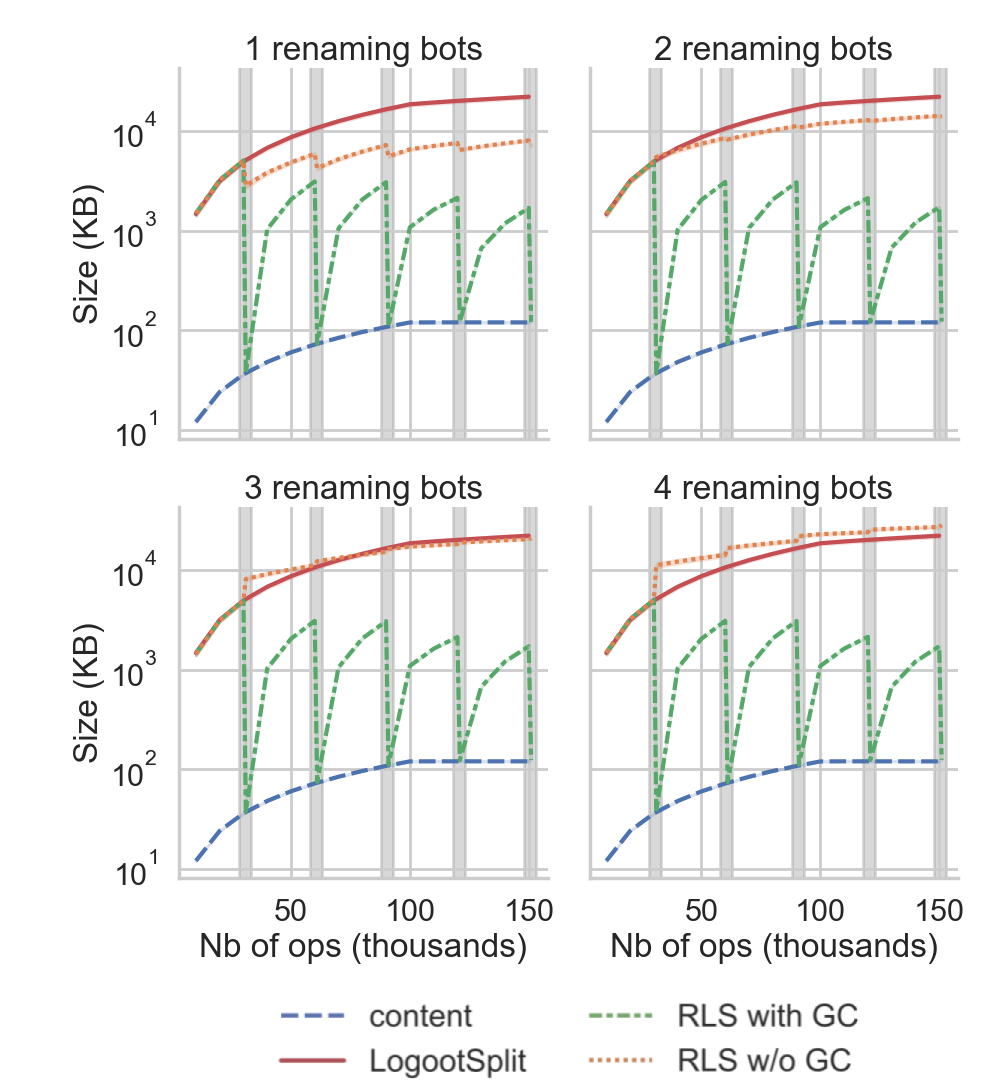
\includegraphics[width=0.7\columnwidth]{img/snapshot-sizes-alt-legende-v2.png}
  \caption{Evolution of the size of the document}
  \label{fig:evolution-document-size}
\end{figure}

Pour chaque graphique dans la \autoref{fig:evolution-document-size}, nous représentons 4 données différentes.
La ligne pointillée bleue correspond à la taille du contenu du document, \ie du texte, tandis que la ligne continue rouge représente la taille complète du document LogootSplit.

La ligne verte en pointillés représente la taille du document RenamableLogootSplit dans son meilleur cas.
Dans ce scénario, les noeuds considèrent que les opérations \emph{rename} sont supprimables dès qu'ils les reçoivent.
Les noeuds peuvent alors bénéficier des effets du mécanisme de renommage tout en supprimant les métadonnées qu'il introduit : les \emph{anciens états} et époques.
Ce faisant, les noeuds peuvent minimiser de manière périodique le surcoût en métadonnées de la structure de données, indépendamment du nombre de \emph{renaming bots} et d'opérations \emph{rename} concurrentes générées.

La ligne pointillée orange représente la taille du document RenamableLogootSplit dans son pire cas.
Dans ce scénario, les noeuds considèrent que les opérations \emph{rename} ne deviennent jamais causalement stables et qu'elles ne peuvent donc jamais être supprimées.
Les noeuds doivent alors conserver de façon permanente les métadonnées introduites par le mécanisme de renommage.
Les performances de RenamableLogootSplit diminuent donc à mesure que le nombre de \emph{renaming bots} et d'opérations \emph{rename} générées augmente.
Néanmoins, nous observons que RenamableLogootSplit peut surpasser les performances de LogootSplit tant que le nombre de \emph{renaming bots} reste faible (1 ou 2).
Ce résultat s'explique par le fait que le mécanisme de renommage permet aux noeuds de supprimer les métadonnées de la structure de données utilisée en interne pour représenter la séquence.

Pour récapituler les résultats présentés, le mécanisme de renommage introduit un surcoût temporaire en métadonnées qui augmente avec chaque opération \emph{rename}.
Mais le surcoût se résorbe à terme une fois que le système devient quiescent et que les opérations \emph{rename} deviennent causalement stables.
Dans la section \autoref{sec:offloading-former-states}, nous détaillerons l'idée que les \emph{anciens états} peuvent être déchargés sur le disque en attendant que la stabilité causale soit atteinte pour atténuer le surcoût temporaire en métadonnées.

\subsubsection{Temps d'intégration des opérations standards}

Nous avons ensuite comparé l'évolution du temps d'intégration des opérations standards, \ie les opérations \emph{insert} et \emph{remove}, sur des documents LogootSplit et RenamableLogootSplit.
Puisque les deux types d'opérations partagent la même complexité temporelle, nous avons seulement utilisé des opérations \emph{insert} dans nos benchmarks.
Nous faisons par contre la différence entre les mises à jours \emph{locales} et \emph{distantes}.
Conceptuellement, les modifications locales peuvent être décomposées comme présenté dans \cite{baquero2017pure} en les deux étapes suivantes :
\begin{enumerate*}[label=(\roman*)]
  \item la génération de l'opération correspondante
  \item l'application de l'opération correspondante sur l'état local.
\end{enumerate*}
Cependant, pour des raisons de performances, nous avons fusionné ces deux étapes dans notre implémentation.
Nous distinguons donc les résultats des modifications \emph{locales} et des modifications \emph{distantes} dans nos benchmarks.
La \autoref{fig:evolution-integration-time-insert} présente les résultats obtenus.

\begin{figure}[!ht]
  \centering
  \subfloat[Local updates]{
      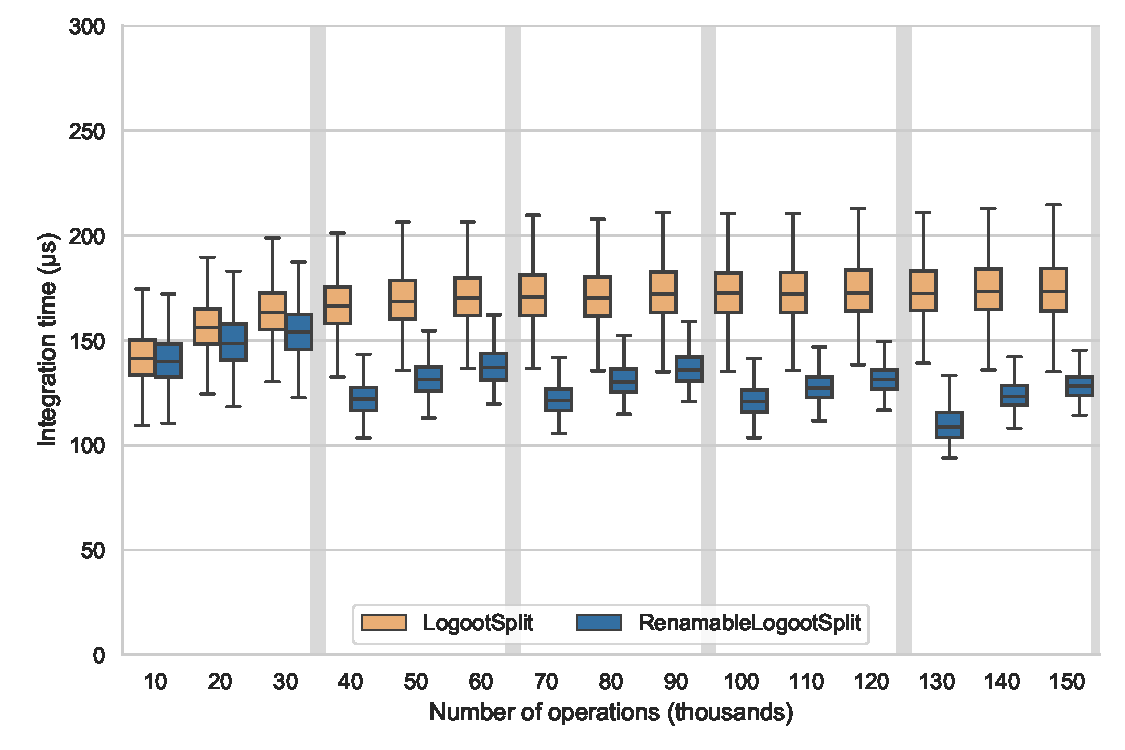
\includegraphics[width=0.45\columnwidth]{img/integration-time-boxplot-local-operations-without-outliers.pdf}
      \label{fig:evolution-integration-time-local-insert}}
  \hfil
  \subfloat[Remote updates]{
      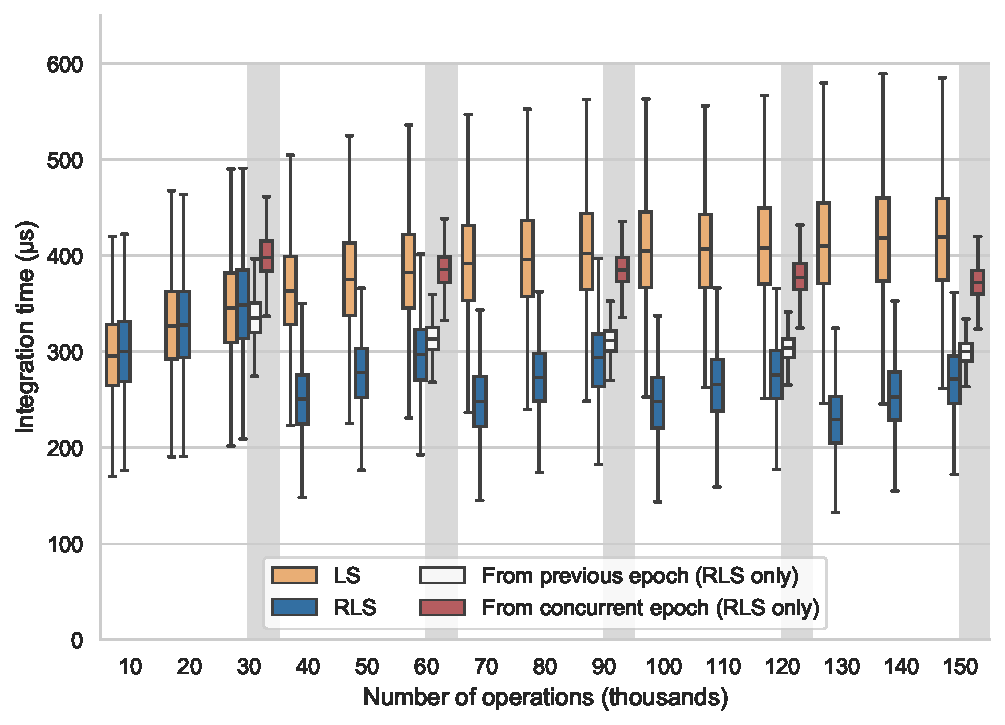
\includegraphics[width=0.45\columnwidth]{img/integration-time-boxplot-remote-operations-without-outliers.pdf}
      \label{fig:evolution-integration-time-remote-insert}}
  \caption{Integration time of standard operations}
  \label{fig:evolution-integration-time-insert}
\end{figure}

Dans ces figures, les boxplots orange correspondent aux temps d'intégration sur des documents LogootSplit, les boxplots bleu sur des documents RenamableLogootSplit.
Bien que les deux mesures soient initialement équivalentes, les temps d'intégration sur des documents RenamableLogootSplit sont ensuite réduits par rapport à ceux de LogootSplit une fois que des opérations \emph{rename} ont été intégrées.
Cette amélioration s'explique par le fait que l'opération \emph{rename} optimise la représentation interne de la séquence.

Dans le cadre des opérations distantes, nous avons mesuré des temps d'intégration spécifiques à RenamableLogootSplit : le temps d'intégration d'opérations distantes provenant d'époques \emph{parentes} et d'époques \emph{soeurs}, respectivement affiché sous la forme de boxplots blanche et rouge dans la \autoref{fig:evolution-integration-time-remote-insert}.

Les opérations distantes provenant d'époques \emph{parentes} sont des opérations générées de manière concurrente à l'opération \emph{rename} mais appliquées après cette dernière.
Puisque l'opération doit être transformée au préalable en utilisant \textsc{renameId}, nous observons un surcoût computationnel par rapport aux autres opérations.
Mais ce surcoût est compensé par l'optimisation de la représentation interne de la séquence effectuée par l'opération \emph{rename}.

Concernant les opérations provenant d'époques \emph{soeurs}, nous observons un surcoût additionnel puisque les noeuds doivent tout d'abord annulé les effets de l'opération \emph{rename} concurrente en utilisant \textsc{revertRenameId}.
À cause de cette étape supplémentaire, les performances de RenamableLogootSplit pour ces opérations sont comparables à celles de LogootSplit.

Pour récapituler, les fonctions de transformation ajoutent un surcoût aux temps d'intégration des opérations concurrentes aux opérations \emph{rename}.
Malgré ce surcoût, RenamableLogootSplit obtient de meilleures performances que LogootSplit tant que la distance entre l'époque de génération de l'opération et l'époque courante du noeud reste limité.
Au fur et à mesure que la distance entre les deux époques augmente, les performances de RenamableLogootSplit diminuent, jusqu'à atteindre des performances moins bonnes que celles de LogootSplit, puisque le surcoût est multiplié.
Néanmoins, le mécanisme de renommage réduit le temps d'intégration de la majorité des opérations, \ie les opérations générées entre deux séries d'opérations \emph{rename}.

\subsubsection{Temps d'intégration de l'opération de renommage}

Finalement, nous avons mesuré l'évolution du temps d'intégration de l'opération \emph{rename} en fonction du nombre d'opérations depuis l'opération \emph{rename} précédente.
Comme précédemment, nous distinguons les performances des modifications \emph{locales} et \emph{distantes}.
Le cas des opérations \emph{rename distantes} se sous-divise en trois catégories.
Les opérations \emph{distantes directes} désignent les opérations \emph{rename distantes} qui introduisent une nouvelle époque \emph{enfant} de l'époque courante du noeud.
Les opérations \emph{concurrentes introduisant une plus grande} (resp. \emph{petite}) \emph{époque} désigne les opérations \emph{rename} qui introduisent une époque \emph{soeur} de l'époque courante du noeud.
D'après la relation \emph{priority}, l'époque introduite est plus grande (resp. petite) que l'époque courante du noeud.
Les résultats obtenus sont présentés dans le \autoref{tab:evolution-integration-time-rename}.

\begin{table}[!ht]
  \centering
  \caption{Integration time of rename operations}
  \label{tab:evolution-integration-time-rename}
  \resizebox{0.7\columnwidth}{!}{
      \begin{tabular}{lrrrrr}
          \toprule
          \multicolumn{2}{c}{Parameters} & \multicolumn{4}{c}{Integration Time (ms)} \\
          \cmidrule(lr){1-2} \cmidrule(lr){3-6}
          Type & Nb Ops (k) &   Mean &   Median & 99\textsuperscript{th} Quant. &    Std \\
          \midrule
          Local & 30  &    41.75 &    38.74 &      71.68 &   6.84 \\
                                  & 60  &    78.32 &    78.16 &      81.42 &   1.24 \\
                                  & 90  &   119.19 &   118.87 &     124.22 &   2.49 \\
                                  & 120 &   143.75 &   143.57 &     148.59 &   2.16 \\
                                  & 150 &   158.04 &   157.95 &     164.38 &   2.49 \\
          \cmidrule(lr){1-6}
          Direct remote & 30  &   481.32 &   477.13 &     537.30 &  17.11 \\
                                  & 60  &   981.62 &   978.24 &    1072.83 &  31.54 \\
                                  & 90  &  1491.28 &  1481.83 &    1657.58 &  51.10 \\
                                  & 120 &  1670.00 &  1663.85 &    1814.38 &  50.29 \\
                                  & 150 &  1694.17 &  1675.95 &    1852.55 &  59.94 \\
          \cmidrule(lr){1-6}
          Cc. int. greater epoch & 30  &   643.53 &   643.57 &     682.80 &  13.42 \\
                                  & 60  &  1317.66 &  1316.39 &    1399.55 &  28.67 \\
                                  & 90  &  1998.23 &  1994.08 &    2111.98 &  45.37 \\
                                  & 120 &  2239.71 &  2233.22 &    2368.45 &  50.06 \\
                                  & 150 &  2241.92 &  2233.61 &    2351.02 &  52.20 \\
          \cmidrule(lr){1-6}
          Cc. int. lesser epoch & 30  &     1.36 &     1.30 &       3.53 &   0.37 \\
                                  & 60  &     2.82 &     2.69 &       4.85 &   0.45 \\
                                  & 90  &     4.45 &     4.23 &       5.81 &   0.71 \\
                                  & 120 &     5.33 &     5.10 &       8.78 &   0.90 \\
                                  & 150 &     5.53 &     5.26 &       8.70 &   0.79 \\
          \bottomrule
      \end{tabular}
  }
\end{table}

Le principal résultat de ces mesures est que les opérations \emph{rename} sont généralement coûteuses quand comparées aux autres types d'opérations, puisque les noeudsd doivent parcourir et renommer leur état courant complet.
Les opérations \emph{rename} locales s'intègrent en plusieurs centaines de millisecondes tandis que les opérations \emph{distantes directes} et \emph{concurrentes introduisant une plus grande époque} peuvent prendre des secondes si retardées trop longtemps.
Il est donc nécessaire de prendre en compte ce résultat pour concevoir des stratégies de génération des opérations \emph{rename} pour éviter d'impacter négativement l'expérience utilisateur.

Un autre résultat intéressant de ces benchmarks est que les opérations \emph{concurrentes introduisant une plus petite époque} sont rapides à intégrer.
Puisque ces opérations introduisent une époque qui n'est pas sélectionné comme nouvelle époque cible, les noeuds ne procède pas au renommage de leur état.
L'intégration des opérations \emph{concurrentes introduisant une plus petite époque} consiste simplement à ajouter l'époque introduite et l'\emph{ancien état} correspondant à l'\emph{arbre des époques}.
Les noeuds peuvent donc réduire de manière significative le coût d'intégration d'un ensemble d'opérations \emph{rename} concurrentes en les appliquant dans l'ordre le plus adapté en fonction du contexte.

\section{Discussion}
\subsection{Implémentation alternative à base d'operation-log}
\subsection{Définition de relations de priorité plus optimales}

Bien que la relation \emph{priority} proposée dans la \autoref{sec:priority} est simple et garantit que tous les noeuds désignent la même époque comme époque cible, elle introduit un surcoût computationnel significatif dans certains cas.
Notamment, cette relation \emph{priority} autorise le cas où un simple noeud, déconnecté de la collaboration depuis longtemps, force l'ensemble des autres noeuds à annuler les opérations \emph{rename} qu'ils ont effectué pendant ce temps car sa propre opération \emph{rename} introduit la nouvelle époque cible.

La relation \emph{priority} devrait donc être conçu pour garantir la convergence des noeuds, mais aussi pour minimiser les calculs effectués globalement par les noeuds du système.
Pour concevoir une relation \emph{priority} efficace, nous pourrions incorporer dans les opérations \emph{rename} des métriques qui représentent l'état du système et le travail accumulé sur le document (nombre de noeuds actuellement à l'époque \emph{parente}, nombre d'opérations générées depuis l'époque parente, taille du document...).
De cette manière, nous pourrions favoriser la branche de l'\emph{arbre des époques} regroupant les collaborateurs les plus actifs et empêcher les noeuds isolés d'imposer leurs opérations \emph{rename}.

Afin d'offrir une plus grande flexibilité dans la conception de la relation \emph{priority}, il est nécessaire de retirer la contrainte interdisant aux noeuds de rejouer une opération \emph{rename}.
Pour cela, un couple de fonctions réciproques doit être proposée pour \textsc{renameId} et \textsc{revertRenameId}.
Une solution alternative est de proposer une implémentation du mécanisme de renommage qui repose sur les identifiants originaux plutôt que sur ceux transformés, par exemple en utilisant le log des opérations.

\subsection{Report de la transition vers la nouvelle epoch principale}

Comme illustré par \autoref{tab:evolution-integration-time-rename}, intégrer des opérations \emph{rename} distantes est généralement coûteux.
Ce traitement peut générer un surcoût computationnel significatif en cas de multiples opérations \emph{rename} concurrentes.
En particulier, un noeud peut recevoir et intégrer les opérations \emph{rename} concurrentes dans l'ordre inverse défini par la relation \emph{priority} sur leur époques.
Dans ce scénario, le noeud considérerait chaque nouvelle époque introduite comme la nouvelle époque cible et renommerait son état en conséquence à chaque fois.

En cas d'un grand nombre d'opérations \emph{rename} concurrentes, nous proposons que les noeuds délaient le renommage de leur état vers l'époque cible jusqu'à ce qu'ils aient obtenu un niveau de confiance donné en l'époque cible.
Ce délai réduit la probabilité que les noeuds n'effectuent des traitements inutiles.
Plusieurs stratégies peuvent être proposées pour calculer le niveau de confiance en l'époque cible.
Ces stratégies peuvent reposer sur une variété de métriques pour produire le niveau de confiance, tel que le temps écoulé depuis que le noeud a reçu une opération \emph{rename} concurrente et le nombre de noeuds en ligne qui n'ont pas encore reçu l'opération \emph{rename}.

Durant cette période d'incertitude introduite par le report, les noeuds peuvent recevoir des opérations provenant d'époques différentes, notamment de l'époque cible.
Néanmoins, les noeuds peuvent toujours intégrer les opérations \emph{insert} et \emph{remove} en utilisant \textsc{renameId} et \textsc{revertRenameId} au prix d'un surcoût computationnel pour chaque identifiant.
Cependant, ce coût est négligeable (plusieurs centaines de microsecondes par identifiant d'après \autoref{fig:evolution-integration-time-remote-insert}) comparé au coût de renommer, de manière inutile, complètement l'état (plusieurs centaines de milliseconds à des secondes complètes d'après \autoref{tab:evolution-integration-time-rename}).

Notons que ce mécanisme nécessite que \textsc{renameId} et \textsc{revertRenameId} soient des fonctions réciproques.
En effet, au cours de la période d'incertitude, un noeud peut avoir à utiliser \textsc{revertRenameId} pour intégrer les identifiants d'opérations \emph{insert} distantes provenant de l'époque cible.
Ensuite, le noeud peut devoir renommer son état vers l'époque cible une fois que celle-ci a obtenu le niveau de confiance requis.
Il s'ensuit que \textsc{renameId} doit restaurer les identifiants précédemment transformés par \textsc{revertRenameId} à leur valeur initiale pour garantir la convergence.

\section{Conclusion}
% \include{assets/chapter_application_HAL}

\NumberThisInToc
\chapter{Stratégies de déclenchement du renommage}
\minitoc
\section{Motivation}
\section{Stratégies proposées}
\subsection{Propriétés}
\subsection{Stratégie 1 : ???}
\subsection{Stratégie 2 : ???}

NOTE: Peut considérer une stratégie où on prend en compte la hauteur de l'epoch tree pour déclencher un renommage : peut attendre qu'on ait plus qu'une epoch pour autoriser un nouveau renommage d'avoir lieu.
Permettrait d'empêcher le cas où un noeud revient après 6 mois d'absence et doit intégrer 100 renommages avant de pouvoir collaborer.
Mais dans le cas où un noeud ne rejoint plus la collaboration, bloque le mécanisme de renommage pour les autres

\section{Évaluation}
\section{Conclusion}
% \include{assets/chapter_extension}

\NumberThisInToc
\chapter{MUTE, un éditeur web collaboratif P2P temps réel}
\minitoc
\section{Présentation}
\subsection{Objectifs}

\begin{itemize}
  \item Éditeur collaboratif
  \item Permettre collaboration synchrone (temps réel) et asynchrone (mode offline)
  \item À grande échelle
  \item Respecter privacy, limiter au maximum la confiance qu'on demande aux utilisateurs d'avoir dans l'outil
  \item Facile d'accès
  \item Facilement déployable par des tiers
  \item S'inscrit dans la mouvance Local-First Software \cite{localfirstsoftware2019,pushpin2020}
\end{itemize}

\subsection{Architecture}

\begin{itemize}
  \item Pour répondre à ces besoins, a effectué les choix suivants
  \item Application web
  \item Utilise CRDT pour représenter le document partagé
  \item Nous permet de supporter les différents modes de collaboration
  \item Nous permet aussi d'adopter une architecture P2P garantissant la privacy et le passage à l'échelle
  \item Mais présence de plusieurs serveurs, aux responsabilités limitées, pour simplifier la collaboration (signaling server, pulsar, bots(?))
  \item \mnnote{TODO: Insérer schéma de l'architecture d'une collaboration (noeuds, types de noeuds et lien)}
  \item L'architecture d'un pair se décompose en plusieurs couches
  \item \mnnote{TODO: Insérer schéma de l'architecture logicielle d'un pair}
\end{itemize}

\section{Couche interface}

\begin{itemize}
  \item Éditeur Markdown
  \item Permet d'incorporer le style des éléments directement dans la séquence représentant le document texte
  \item Mécanisme de conscience de groupe
  \begin{itemize}
    \item Liste des collaborateurs
    \item Curseurs et sélections des autres collaborateurs
    \item Indicateur de connexion
  \end{itemize}
  \item Stocke au sein du navigateur les données du document (état du document, log des opérations...)
  \item Glue le reste des couches ensemble
\end{itemize}

\section{Couche réplication}
\subsection{Document texte}

\begin{itemize}
  \item Implémentation de RenamableLogootSplit que nous avons réutilisé dans le cadre de nos simulations et évaluations
  \item Associée au composant gérant la livraison des opérations
  \item Mécanisme d'anti-entropie \cite{1983-anti-entropy-vv}
\end{itemize}

\subsection{Métadonnées}

\begin{itemize}
  \item Titre (Simple LWW-Register)
  \item Mode de chiffrement (fixe)
\end{itemize}

\subsection{Collaborateurs}

\begin{itemize}
  \item Implémente Swim \cite{swim2002}
  \item Découple protocole de détection des failures du protocole de diffusion de l'évolution du groupe
  \item Protocole de détection des failures
    \begin{itemize}
      \item Basé sur un système de rounds, basés sur un interval de temps
      \item À chaque round, chaque pair probe de manière aléatoire un autre pair
      \item Si pas de réponse, demande à un autre pair de le contacter
      \item Si pas de réponse par leur intermédiaire, pair devient suspect
      \item Si toujours pas de nouvelles du pair après un certain temps, le considère déconnecté
    \end{itemize}
  \item Protocole de diffusion de l'évolution du groupe
    \begin{itemize}
      \item Plutôt que de diffuser chaque évolution du groupe, adopte un modèle de diffusion épidémique
      \item Piggyback les évolutions aux messages du protocole de détection des failures
    \end{itemize}
  \item Modifie le fonctionnement du protocole pour en faire un CRDT
  \item Afin de permettre un nouveau pair de récupérer instantanément état courant du groupe
  \item Autorise aussi un pair à se déconnecter puis reconnecter en modifiant l'ordre de priorité entre les différents messages
  \begin{itemize}
    \item Dans protocole original, un pair déconnecté doit revenir sous une nouvelle identité
    \item Afin de maintenir l'identifiant du pair, notamment pour ses opérations sur le document
  \end{itemize}
\end{itemize}

\subsection{Curseurs}

\begin{itemize}
  \item Repose sur des identifiants pour indiquer la position des curseurs
  \item Vecteur de LWW-Registers, chaque LWW-Register étant associé à un pair actuellement connecté
\end{itemize}

\section{Couche sécurité}
\subsection{Authenticité des clés publiques des participants}
\begin{itemize}
  \item Trusternity \cite{2018-trusternity-short, 2018-trusternity-long}
\end{itemize}

\subsection{Établissement de la clé de chiffrement de groupe}
\begin{itemize}
  \item n-party Diffie-Hellman \cite{1995-diffie-hellman}
\end{itemize}

\section{Couche réseau}
\subsection{Netflux}
\begin{itemize}
  \item Réseau P2P
  \item Interface uniforme permettant d'interagir à la fois avec des navigateurs et des bots
  \item Connectent les noeuds en utilisant la technologie WebRTC
  \item Connectent les bots en utilisant la technologie WebSocket
  \item Repose sur l'utilisation d'un signaling server pour permettre aux pairs de rejoindre la collaboration
  \item Topologie maillée
\end{itemize}
\subsection{Pulsar}
\begin{itemize}
  \item Log-based message broker
  \item Propose plusieurs modes de fonctionnement
  \item En mode log-based message broker, maintient l'ensemble des messages reçus dans un log
  \item Permet, lorsque utilisé pour diffuser les opérations, de conserver le log complet des opérations
  \item Permet alors à un nouveau noeud de récupérer l'ensemble des opérations connues et de reconstruire l'état courant du document, même si actuellement aucun autre pair n'est connecté
  \item En mode message broker, diffuse seulement les messages aux noeuds actuellement connectés au topic
  \item Permet de communiquer les messages transients (protocole d'établissement de la clé de groupe, heartbeat de Swim, mécanisme d'anti-entropie du document) sans polluer le log
  \item Pose néanmoins des questions de sécurité et d'utilisabilité
  \item Besoin de chiffrer E2E les opérations
  \item Dans ce cas
    \begin{itemize}
      \item comment un nouveau pair peut obtenir la clé de chiffrement si les autres pairs ne sont pas connectés ? (à moins de revenir à un chiffrement à base de passphrase, avec les problèmes qui en découlent)
      \item comment un nouveau pair peut relire les opérations chiffrer avec l'ancienne clé ?
    \end{itemize}
\end{itemize}

\section{Pistes d'amélioration et de recherche}

\subsection{Composition de CRDTs}

\begin{itemize}
  \item
\end{itemize}

\subsection{CRDT pour les styles}

\begin{itemize}
  \item Permettrait de se découpler de Markdown pour gérer le style du document
  \item Permettrait de supporter un plus grand nombre d'options que Markdown ne le permet actuellement (couleurs, mise en page...)
\end{itemize}

\subsection{Réseaux}
\begin{itemize}
  \item Librairies alternatives (libP2P, hypercore)
  \item Topologies alternatives (SPRAY)
\end{itemize}
\subsection{Évolution de schéma}
\begin{itemize}
  \item Cambria \cite{2021-cambria-schema-evolution}
\end{itemize}
\subsection{Droits d'accès}
\begin{itemize}
  \item Access Control Conflict Resolution in Distributed File Systems \cite{2021-access-control-crdts}
  \item Travaux de PA
\end{itemize}
\subsection{Historique du document}
\subsection{Rôles et places des bots dans systèmes collaboratifs}
\begin{itemize}
  \item Stockage du document pour améliorer sa disponibilité
  \item Overleaf en P2P ?
  \item Comment réinsérer des bots dans la collaboration sans en faire des éléments centraux, sans créer des failles de confidentialité, et tout en rendant ces fonctionnalités accessibles ?
\end{itemize}

\NumberThisInToc
\chapter{Conclusions et perspectives}
\minitoc
\section{Résumé des contributions}
\section{Perspectives}
\subsection{Définition de relations de priorité plus optimales}
\subsection{Redéfinition de la sémantique du renommage en déplacement d'éléments}
\subsection{Définition de types de données répliquées sans conflits plus complexes}
% \NumberThisInToc
\chapter{Conclusions et perspectives}
\minitoc
\label{chap:conclusions-perspectives}

Dans ce chapitre, nous revenons sur les contributions présentées dans cette thèse.
Nous rappelons le contexte dans lequel elles s'inscrivent, récapitulons leurs spécificités et apports, et finalement précisons plusieurs de leurs limites.
Puis, nous concluons ce manuscrit en présentant plusieurs pistes de recherche qui nous restent à explorer à l'issue de cette thèse.
La première s'inscrit dans la continuité directe de nos travaux sur un mécanisme de ré-identification pour \acp{CRDT} pour le type Séquence pour les applications \acf{LFS}.
Les dernières traduisent quant à elles notre volonté de recentrer nos travaux sur le domaine plus général des \acp{CRDT}.


\section{Résumés des contributions}

\subsection{Réflexions sur l'état de l'art des \acp{CRDT}}
Les \acfp{CRDT} \cite{shapiro_2011_crdt} sont de nouvelles spécifications des types de données.
Ils sont conçus pour permettre à un ensemble de noeuds d'un système de répliquer une même donnée et pour leur permettre de la consulter et de la modifier sans aucune coordination préalable.
Les copies des noeuds divergent alors temporairement.
Les noeuds se synchronisent ensuite pour s'échanger leurs modifications respectives.
Les \acp{CRDT} garantissent alors la cohérence forte à terme \cite{shapiro_2011_crdt}, \ie que les noeuds obtiennent de nouveau des copies équivalentes de la donnée.

L'absence de coordination entre les noeuds avant modifications implique que des noeuds peuvent modifier la donnée en concurrence.
De telles modifications peuvent donner lieu à des conflits, \eg l'ajout et la suppression en concurrence d'un même élément dans un ensemble.
Pour pallier ce problème, les \acp{CRDT} incorporent un mécanisme de résolution de conflits automatiques directement au sein de leur spécification.

Il convient de noter qu'il existe plusieurs solutions possibles pour résoudre un conflit.
Pour reprendre l'exemple de l'élément ajouté et supprimé en concurrence d'un ensemble, nous pouvons par exemple soit le conserver l'élément, soit le supprimer.
Nous parlons alors de sémantique du mécanisme de résolution de conflits automatique.

De la même manière, il existe plusieurs approches possibles pour synchroniser les noeuds, \eg diffuser chaque modification de manière atomique ou diffuser l'entièreté de l'état périodiquement.
Ainsi, lors de la définition d'un \ac{CRDT}, il convient de préciser les sémantiques de résolution de conflits qu'il adopte et le modèle de synchronisation qu'il utilise \cite{2018-crdts-overview-preguica}.\\

Depuis leur formalisation, de nombreux travaux ont abouti à la conception de nouveaux \acp{CRDT}, soit en spécifiant de nouvelles sémantiques de résolution de conflits pour un type de données \cite{2020-cl-set-weihai}, soit en spécifiant de nouveaux modèles de synchronisation \cite{Almeida_2018} ou en enrichissant les spécifications des modèles existants \cite{baquero2017pure,enes2019}.

Dans notre présentation des \acp{CRDT} \cf{sec:etat-art-crdts-intro}, nous présentons chacun de ces aspects.
Cependant, nous nous ne limitons pas à retranscrire l'état de l'art de la littérature.
Notamment au sujet du modèle de synchronisation par opérations, nous précisons que le modèle de livraison causal n'est pas nécessaire pour l'ensemble des \acp{CRDT} synchronisés par opérations, \ie que certains peuvent adopter des modèles de livraison moins contraints et donc moins coûteux.
Cette précision nous permet de proposer une étude comparative des différents modèles de synchronisation qui est, à notre connaissance, l'une des plus précises de la littérature \cf{def:synchro-synthese}.\\

Nous présentons ensuite les différents \acp{CRDT} pour le type Séquence de la littérature \cf{sec:seq-crdts}.
Nous mettons alors en exergue les deux approches proposées pour concevoir le mécanisme de résolution de conflits automatiques pour le type Séquence, \ie l'approche à pierres tombales et l'approche à identifiants densément ordonnés.
De nouveau, cette rétrospective nous permet d'expliciter des angles morts des articles d'origine, notamment vis-à-vis des modèle de livraison des opérations des \acp{CRDT} proposés.
Puis, nous mettons en lumière les limites des évaluations comparant les deux approches, \ie le couplage entretenu entre approche du mécanisme de résolution de conflits et choix d'implémentations.
Cette limite empêche d'établir la supériorité d'une des approches par rapport à l'autre.
Finalement, nous conjecturons que le surcoût de ces deux approches est le même, \ie le coût nécessaire à la représentation d'un espace dense.
Nous précisons dès lors par le biais de notre propre étude comparative comment ce surcoût s'exprime dans chacune des approches , \ie le compromis entre surcoût en métadonnées, calculs et bande-passante proposé par les deux approches \cf{sec:seq-crdts-synth}.\\

Ces réflexions que nous présentons sur l'état des \acp{CRDT} définissent plusieurs pistes de recherches.
Une première d'entre elles concerne notre étude comparative des modèles de synchronisation.
D'après les critères que nous utilisons, une conclusion possible de cette comparaison est que le modèle de synchronisation par différences d'états rend obsolètes les modèles de synchronisation par états et par opérations.
En effet, le modèle de synchronisation par différences d'états apparaît comme adapté à l'ensemble des contextes d'utilisation qui étaient jusqu'alors exclusifs à ces derniers, de par les multiples stratégies qu'il permet, \eg synchronisation par états complets, synchronisation par états irréductibles...

Cette conclusion nous paraît cependant hâtive.
Il convient d'étendre notre étude comparative pour prendre en compte des critères de comparaison additionnels pour confirmer cette conjecture, ou l'invalider et définir plus précisément les spécificités de chacun des modèles de synchronisation.
Nous détaillons cette piste de recherche dans la \autoref{sec:perspective-comparison-sync-models}.\\

Une seconde piste de recherche possible concerne les deux approches utilisées pour concevoir le mécanisme de résolution de conflits des \acp{CRDT} pour le type Séquence.
Comme dit précédemment, nous conjecturons que ces deux approches ne sont finalement que deux manières différentes de représenter une même information : la position d'un élément dans un espace dense.
La différence entre ces approches résiderait uniquement dans la manière que chaque représentation influe sur les performances du \ac{CRDT}.
Une piste de travail serait donc de confirmer cette conjecture, en proposant une formalisation unique des \acp{CRDT} pour le type Séquence.


\subsection{Ré-identification sans coordination pour les \acp{CRDT} pour le type Séquence}
Pour privilégier leur disponibilité, latence et tolérance aux pannes, les systèmes distribués peuvent adopter le paradigme de la réplication optimiste \cite{2005-optimistic-replication-saito}.
Ce paradigme consiste à relaxer la cohérence de données entre les noeuds du système pour leur permettre de consulter et modifier leur copie locale sans se coordonner.
Leur copies peuvent alors temporairement diverger avant de converger de nouveau une fois les modifications de chacun propagées.
Cependant, cette approche nécessite l'emploi d'un mécanisme de résolution de conflits pour assurer la convergence même en cas de modifications concurrentes.
Pour cela, l'approche des \acp{CRDT} \cite{2007-crdt-shapiro,shapiro_2011_crdt} propose d'utiliser des types de données dont les modifications sont nativement commutatives.

Depuis la spécification des \acp{CRDT}, la littérature a proposé plusieurs de ces mécanismes résolution de conflits automatiques pour le type de données Séquence \cite{2006-woot-oster,ROH2011354,2009-treedoc-preguica,2009-logoot-weiss}.
Cependant, ces approches souffrent toutes d'un surcoût croissant de manière monotone.
Ce problème a été identifié par la communauté, et celle-ci a proposé pour y répondre des mécanismes permettant soit de réduire la croissance du surcoût \cite{lseq2013,lseq2017}, soit d'effectuer une \ac{GC} du surcoût \cite{ROH2011354,letia:hal-01248270,zawirski:hal-01248197}.
Nous avons cependant déterminé que ces mécanismes ne sont pas adaptés aux systèmes \ac{P2P} à large échelle souffrant de churn et utilisant des \acp{CRDT} pour Séquence à granularité variable.

Dans le cadre de cette thèse, nous avons donc souhaité proposer un nouveau mécanisme adapté à ce type de systèmes.
Pour cela, nous avons suivi l'approche proposée par \cite{letia:hal-01248270,zawirski:hal-01248197} : l'utilisation d'un mécanisme pour ré-assigner de nouveaux identifiants aux élements stockées dans la séquence.
Nous avons donc proposé un nouveau mécanisme appartenant à cette approche pour le \ac{CRDT} LogootSplit \cite{2013-logootsplit}.\\

Notre proposition prend la forme d'un nouvel \ac{CRDT} pour Séquence à granularité variable : RenamableLogootSplit.
Ce nouveau \ac{CRDT} associe à LogootSplit un nouveau type de modification, $\trm{ren}$, permettant de produire une nouvelle séquence équivalente à son état précédent.
Cette nouvelle modification tire profit de la granularité variable de la séquence pour produire un état de taille minimale : elle assigne à tous les éléments des identifiants de position issus d'un même intervalle.
Ceci nous permet de minimiser les métadonnées que la séquence doit stocker de manière effective.
% De plus, le passage à une représentation interne minimale de la séquence nous permet d'améliorer le coût des modifications suivantes en termes de calculs.

Afin de gérer les opérations concurrentes aux opérations $\trm{ren}$, nous définissons pour ces dernières un algorithme de transformation.
Pour cela, nous définissons un mécanisme d'époques nous permettant d'identifier la concurrence entre opérations.
De plus, nous introduisons une relation d'ordre strict total, \emph{priority}, pour résoudre de manière déterministe le conflit provoqué par deux opérations $\trm{ren}$, \ie pour déterminer quelle opération $\trm{ren}$ privilégier.
Finalement, nous définissons deux algorithmes, \texttt{renameId} et \texttt{revertRenameId}, qui permettent de transformer les opérations concurrentes à une opération $\trm{ren}$ pour prendre en compte l'effet de cette dernière.
Ainsi, notre algorithme permet de détecter et de transformer les opérations concurrentes aux opérations $\trm{ren}$, sans nécessiter une coordination synchrone entre les noeuds.\\


Pour valider notre approche, nous proposons une évaluation expérimentale de cette dernière.
Cette évaluation se base sur des traces de sessions d'édition collaborative que nous avons généré par simulations.
Chacune de ces simulations représente la rédaction collaborative d'un document texte par 10 noeuds.

Notre évaluation nous permet de valider de manière empirique les résultats attendus.
Le premier d'entre eux concerne la convergence des noeuds.
En effet, nos simulations nous ont permis de valider que l'ensemble des noeuds obtenaient des états finaux équivalents, même en cas d'opérations $\trm{ren}$ concurrentes.

Notre évaluation nous a aussi permis de valider que le mécanisme de renommage réduit à une taille minimale le surcoût du mécanisme de résolution de conflits incorporé dans le \ac{CRDT} pour Séquence.

L'évaluation expérimentale nous a aussi permis de prendre conscience d'effets additionnels du mécanisme de renommage que nous n'avions pas anticipé.
Notamment, elle montre que le surcoût éventuel du mécanisme de renommage, notamment en termes de calculs, est toutefois contrebalancé par l'amélioration précisée précédemment, \ie la réduction de la taille de la séquence.\\

Finalement, notons que le mécanisme que nous proposons est partiellement générique : il peut être adapté à d'autres \acp{CRDT} pour Séquence à granularité variable, \eg un \ac{CRDT} pour Séquence appartenant à l'approche à pierres tombales.
Dans le cadre d'une telle démarche, nous pourrions réutiliser le système d'époques, la relation \emph{priority} et l'algorithme de contrôle qui identifie les transformations à effectuer.
Pour compléter une telle adaptation, nous devrions cependant concevoir de nouveaux algorithmes \texttt{renameId} et \texttt{revertRenameId} spécifiques et adaptés au \ac{CRDT} choisi.\\

Le mécanisme de renommage que nous présentons souffre néanmoins de plusieurs limites.
La première d'entre elles concerne ses performances.
En effet, notre évaluation expérimentale a mis en lumière le coût important en l'état de la modification $\trm{ren}$ par rapport aux autres modifications en termes de calculs \cf{sec:integration-time-rename}.
De plus, chaque opération $\trm{ren}$ comporte une représentation de l'ancien état qui doit être maintenue par les noeuds jusqu'à leur stabilité causale.
Le surcoût en métadonnées introduit par un ensemble d'opérations $\trm{ren}$ concurrentes peut donc s'avérer important, voire pénalisant \cf{sec:evaluation-metadata}.
Pour répondre à ces problèmes, nous identifions trois axes d'amélioration :
\begin{enumerate}
    \item La définition de stratégies de déclenchement du renommage efficaces.
        Le but de ces stratégies serait de déclencher le mécanisme de renommage de manière fréquente, de façon à garder son temps d'exécution acceptable, mais tout visant à minimiser la probabilité que les noeuds produisent des opérations $\trm{ren}$ concurrentes, de façon à minimiser le surcoût en métadonnées.
    \item La définition de relations \emph{priority} efficaces.
        Nous développons ce point dans la \autoref{sec:alternative-priority}.
    \item La proposition d'algorithmes de renommage efficaces.
        Cette amélioration peut prendre la forme de nouveaux algorithmes pour \texttt{renameId} et \texttt{revertRenameId} offrant une meilleure complexité en temps.
        Il peut aussi s'agir de la conception d'une nouvelle approche pour renommer l'état et gérer les modifications concurrentes, \eg un mécanisme de renommage basé sur le journal des opérations \cf{sec:log-based-rename-mechanism}.
\end{enumerate}

Une seconde limite de RenamableLogootSplit que nous identifions concerne son mécanisme de \ac{GC} des métadonnées introduites par le mécanisme de renommage.
En effet, pour fonctionner, ce dernier repose sur la stabilité causale des opérations $\trm{ren}$.
Pour rappel, la stabilité causale représente le contexte causal commun à l'ensemble des noeuds du système.
Pour le déterminer, chaque noeud doit récupérer le contexte causal de l'ensemble des noeuds du système.
Ainsi, l'utilisation de la stabilité causale comme pré-requis pour la \ac{GC} de métadonnées constitue une contrainte forte, voire prohibitive, dans les systèmes \ac{P2P} à large échelle sujet au churn.
En effet, un noeud du système déconnecté de manière définitive suffit pour empêcher la stabilité causale de progresser, son contexte causal étant alors indéterminé du point de vue des autres noeuds.
Il s'agit toutefois d'une limite récurrente des mécanismes de \ac{GC} distribués et asynchrones \cite{ROH2011354,baquero2017pure,2018-prunable-authenticated-log-vic}.
Nous présentons une piste de travail possible pour pallier ce problème dans la \autoref{sec:manual-merge}.


\subsection{Éditeur de texte collaboratif \ac{P2P} chiffré de bout en bout}
Les applications collaboratives permettent à des utilisateur-rices de réaliser collaborativement une tâche.
Elles permettent à plusieurs utilisateur-rices de consulter la version actuelle du document, de la modifier et de partager leurs modifications avec les autres.
Ceci permet de mettre en place une réflexion de groupe, ce qui améliore la qualité du résultat produit \cite{2004-empirical-study-collaborative-writing,2005-internet-encyclopaedias-head-to-head}.

Cependant, les applications collaboratives sont historiquement des applications centralisées, \eg Google Docs \cite{gdocs}.
Ce type d'architecture induit des défauts d'un point de vue technique, \eg faible capacité de passage à l'échelle et faible tolérance aux pannes, mais aussi d'un point de vue utilisateur, \eg perte de la souveraineté des données et absence de garantie de pérennité.\\

Les travaux de l'équipe Coast s'inscrivent dans une mouvance souhaitant résoudre ces problèmes et qui a conduit à la définition d'un nouveau paradigme d'applications : les applications \acf{LFS} \cite{localfirstsoftware2019}.
Le but de ce paradigme est la conception d'applications collaboratives, \ac{P2P}, pérennes et rendant la souveraineté de leurs données aux utilisateur-rices.

Dans le cadre de cette démarche, l'équipe Coast développe depuis plusieurs années l'application \acf{MUTE}, un éditeur de texte web collaboratif \ac{P2P} temps réel chiffré de bout en bout.
Cette application sert à la fois de plateforme de démonstration et de recherche pour les travaux de l'équipe, mais aussi de \acf{PoC} pour les \ac{LFS}.
Ainsi, \ac{MUTE} propose au moment où nous écrivons ces lignes un aperçu des travaux de recherche existants concernant :
\begin{enumerate}
    \item Les mécanismes de résolution de résolutions de conflits automatiques pour l'édition collaborative de documents textes \cite{2013-logootsplit,2021-these-vic,2022-rls-tpds-nicolas}.
    \item Les protocoles distribués d'appartenance au groupe \cite{swim2002}.
    \item Les mécanismes d'anti-entropie \cite{1983-anti-entropy-vv}.
    \item Les protocoles distribués d'authentification d'utilisateur-rices \cite{2018-trusternity-short,2018-trusternity-long}.
    \item Les protocoles distribués d'établissement de clés de chiffrement de groupe \cite{1995-burmester-desmedt}.
    \item Les mécanismes de conscience de groupe.
\end{enumerate}
Dans cette liste, nous avons personnellement contribué à l'implémentation des \acp{CRDT} LogootSplit \cite{2013-logootsplit} et RenamableLogootSplit \cite{2022-rls-tpds-nicolas}, et du protocole d'appartenance au groupe SWIM \cite{swim2002}.\\

En son état actuel, \ac{MUTE} présente cependant plusieurs limites.
Tout d'abord, l'environnement web implique un certain nombre de contraintes, notamment au niveau des technologies et protocoles disponibles.
Notamment, le protocole \acf{WebRTC} repose sur l'utilisation de serveurs de signalisation, \ie de points de rendez-vous des pairs, et de serveurs de relais, \ie d'intermédiaires pour communiquer entre pairs lorsque les configurations de leur réseaux respectifs interdisent l'établissement d'une connexion directe.
Ainsi, les applications \ac{P2P} web doivent soit déployer et maintenir leur propre infrastructure de serveurs, soit reposer sur une infrastructure existante, \eg celle proposée par OpenRelay \cite{openrelay}.

Dans le cadre de \ac{MUTE}, nous avons opté pour cette seconde solution.
Cependant, ce choix introduit un \acf{SPOF}\footnote{\acf{SPOF} : Point de défaillance unique} dans \ac{MUTE} : OpenRelay elle-même.
Afin de garantir la pérennité de \ac{MUTE}, nous devrions reposer non pas sur une unique infrastructure de serveurs de signalisation et de relais mais sur une multitude.
Malheureusement, l'écosystème actuel brille par la rareté d'infrastructures publiques offrant ces services.
Nous devons donc encourager et supporter la mise en place de telles infrastructures par une pluralité d'organisations.\\

Une autre limite de ce système que nous identifions concerne l'utilisabilité des systèmes \ac{P2P} de manière générale.
L'expérience vécue suivante constitue à notre avis un exemple éloquent des limites actuelles de l'application \ac{MUTE} dans ce domaine.
Après avoir rédigé une version initiale d'un document, nous avons envoyé le lien du document à notre collaborateur pour relecture et validation.
Lorsque notre collaborateur a souhaité accéder au document, celui-ci s'est retrouvé devant une page blanche : comme nous nous étions déconnecté du système entretemps, plus aucun pair possédant une copie n'était disponible pour se synchroniser.

Notre collaborateur était donc dans l'incapacité de récupérer le document et d'effectuer sa tâche.
Afin de pallier ce problème, une solution possible est de faire reposer \ac{MUTE} sur un réseau \ac{P2P} global, \eg le réseau de \ac{IPFS} \cite{ipfs}, et d'utiliser les pairs de ce dernier, potentiellement des pairs étrangers à l'application, comme pairs de stockage pour permettre une synchronisation future.
Cette solution limiterait ainsi le risque qu'un pair ne puisse récupérer l'état du document faute de pairs disponibles.
Pour garantir l'utilisabilité du système \ac{P2P}, une telle solution devrait donc permettre à un pair de récupérer l'état du document à sa reconnexion, malgré la potentielle évolution du groupe des collaborateur-rices et des pairs de stockage, \eg l'ajout, l'éviction ou la déconnexion d'un des pairs.
Cependant, la solution devrait en parallèle garantir qu'elle n'introduit aucune vulnérabilité, \eg la possibilité pour les pairs de stockage selectionnés de reconstruire et consulter le document.
% \item Finalement, une dernière limite que nous identifions est la pérennité économique de ce type d'applications.
%     Selon nous, les systèmes \ac{P2P} chiffrés de bout en bout s'interdisent les modèles économiques dominants et acceptés par les organisations et utilisateur-rices, \ie la collecte et revente de données.
%     En effet,
%     , de par les propriétés qu'ils assurent, notamment la confidentialité des données .
%     \mnnote{TODO: Voir si on a des données sur les entreprises/organisations encourageant le chiffrement de bout-en-bout dans leurs outils internes, }


\section{Perspectives}

\subsection{Définition de relations de priorité pour minimiser les traitements}
\label{sec:alternative-priority}

Dans la \autoref{sec:priority}, nous avons spécifié la relation \emph{priority} \cf{def:priority-relation}.
Pour rappel, cette relation doit établir un ordre strict total sur les époques de notre mécanisme de renommage.

Cette relation nous permet ainsi de résoudre le conflit provoqué par la génération de modifications $\trm{ren}$ concurrentes en les ordonnant.
Grâce à cette relation relation d'ordre, les noeuds peuvent déterminer vers quelle époque de l'ensemble des époques connues progresser.
Cette relation permet ainsi aux noeuds de converger à une époque commune à terme.\\

La convergence à terme à une époque commune présente plusieurs avantages :
\begin{enumerate}
    \item Réduire la distance entre les époques courantes des noeuds, et ainsi minimiser le surcoût en calculs par opération du mécanisme de renommage.
        En effet, il n'est pas nécessaire de transformer une opérations livrée avant de l'intégrer si celle-ci provient de la même époque que le noeud courant.
    \item Définir un nouveau \acf{LCA} entre les époques courantes des noeuds.
        Cela permet aux noeuds d'appliquer le mécanisme de \ac{GC} pour supprimer les époques devenues obsolètes et leur anciens états associés, pour ainsi minimiser le surcoût en métadonnées du mécanisme de renommage.
\end{enumerate}

Il existe plusieurs manières pour définir la relation \emph{priority} tout en satisfaisant les propriétés indiquées.
Dans le cadre de ce manuscrit, nous avons utilisé l'ordre lexicographique sur les chemins des époques dans l'\emph{arbre des époques} pour définir \emph{priority}.
Cette approche se démarque par :
\begin{enumerate}
    \item Sa simplicité.
    \item Son surcoût limité, \ie cette approche n'introduit pas de métadonnées supplémentaires à stocker et diffuser, et l'algorithme de comparaison utilisé est simple.
    \item Sa propriété arrangeante sur les déplacements des noeuds dans l'arbre des époques.
        De manière plus précise, cette définition de \emph{priority} impose aux noeuds de se déplacer que vers l'enfant le plus à droite de l'arbre des époques.
        Ceci empêche les noeuds de faire un aller-retour entre deux époques données.
        Cette propriété permet de passer outre une contrainte concernant le couple de fonctions \texttt{renameId} et \texttt{revertRenameId} : leur reciprocité.
\end{enumerate}

Cette définition présente cependant plusieurs limites.
La limite que nous identifions est sa décorrélation avec le coût et le bénéfice de progresser vers l'époque cible désignée.
En effet, l'époque cible est désignée de manière arbitraire par rapport à sa position dans l'arbre des époques.
Il est ainsi possible que progresser vers cette époque détériore l'état de la séquence, \ie augmente la taille des identifiants et augmente le nombre de blocs.
De plus, la transition de l'ensemble des noeuds depuis leur époque courante respective vers cette nouvelle époque cible induit un coût en calculs, potentiellement important \cf{fig:worst-case-priority}.\\

Pour pallier ce problème, il est nécessaire de proposer une définition de \emph{priority} prenant l'aspect efficacité en compte.
L'approche considérée consisterait à inclure dans les opérations $\trm{ren}$ une ou plusieurs métriques qui représente le travail accumulé sur la branche courante de l'arbre des époques, \eg le nombre d'opérations intégrées, les noeuds actuellement sur cette branche...
L'ordre strict total entre les époques serait ainsi construit à partir de la comparaison entre les valeurs de ces métriques de leur opération $\trm{ren}$ respective.

Il conviendra d'adjoindre à cette nouvelle définition de \emph{priority} un nouveau couple de fonctions \texttt{renameId} et \texttt{revertRenameId} respectant la contrainte de réciprocité de ces fonctions, ou de mettre en place une autre implémentation du mécanisme de renommage ne nécessitant pas cette contrainte, telle qu'une implémentation basée sur le journal des opérations \cf{sec:log-based-rename-mechanism}.

Il conviendra aussi d'étudier la possibilité de combiner l'utilisation de plusieurs relations \emph{priority} pour minimiser le surcoût global du mécanisme de renommage, \eg en fonction de la distance entre deux époques.

Finalement, il sera nécessaire de valider l'approche proposée par une évaluation comparative par rapport à l'approche actuelle.
Cette évaluation pourrait consister à monitorer le coût du système pour observer si l'approche proposée permet de réduire les calculs de manière globale.
Plusieurs configurations de paramètres pourraient aussi être utilisées pour déterminer l'impact respectif de chaque paramètre sur les résultats.


% \subsection{Détection et fusion manuelle de versions distantes}
% \begin{itemize}
    \item Est-ce que ça a vraiment du sens d'intégrer automatiquement des modifications ayant été généré sur une version du document distante de l'état actuel du document (voir distance de Hamming, Levenstein, String-to-string correction problem (Tichy et al))
    \item Jusqu'à quelle distance est-ce que la fusion automatique a encore du sens ?
    \mnnote{NOTE: Peut connecter ça à la nécessité de conserver un chemin d'une époque à l'autre : si les opérations émises depuis cette époque ont probablement plus d'intérêt pour l'état actuel, couper l'arbre ?}
  \end{itemize}


\subsection{Étude comparative des différents modèles de synchronisation pour \acp{CRDT}}
\begin{itemize}
  \item Comme évoqué dans l'état de l'art \cf{sec:delta-crdts}, un nouveau modèle de synchronisation pour \ac{CRDT} fut proposé récemment \cite{almeida2015delta}.
    Ce dernier propose une synchronisation des noeuds par le biais de différences d'états.
  \item Pour rappel, ce nouveau modèle de synchronisation se base sur le modèle de synchronisation par états.
    Il partage les mêmes pré-requis, à savoir la nécessité d'une fonction \texttt{merge} associative, commutative et idempotente.
    Cette dernière doit permettre de la fusion toute paire d'états possible en calculant leur borne supérieure, \ie leur \ac{LUB}.
  \item La spécificité de ce nouveau modèle de synchronisation est de calculer pour chaque modification la différence d'état correspondante.
    Cette différence correspond à un élément irréductible du sup-demi-treillis du \ac{CRDT} \cite{enes2019}, \ie un état particulier de ce dernier.
    Cet élément irréductible peut donc être diffusé et intégré par les autres noeuds, toujours à l'aide de la fonction \texttt{merge}.
  \item Ce modèle de synchronisation permet alors d'adopter une variété de stratégies de synchronisation, \eg diffusion des différences de manière atomique, fusion de plusieurs différences puis diffusion du résultat..., et donc de répondre à une grande variété de cas d'utilisation.
  \item Dans notre comparaison des modèles de synchronisation \cf{def:synchro-synthese}, nous avons justifié que les \acp{CRDT} synchronisés par différences d'états peuvent être utilisés dans les mêmes contextes que les \acp{CRDT} synchronisés par états et que les \acp{CRDT} synchronisés par opérations.
    Cette conclusion nous mène à reconsidérer l'intérêt des autres modèles de synchronisation de nos jours.
  \item Par exemple, un \ac{CRDT} synchronisé par différences d'états correspond à un \ac{CRDT} synchronisé par états dont nous avons identifié les éléments irréductibles.
    La différence entre ces deux modèles de synchronisation semble reposer seulement sur la possibilité d'utiliser ces éléments irréductibles pour propager les modifications, en place et lieu des états complets.
    Nous conjecturons donc que le modèle de synchronisation par états est rendu obsolète par celui par différences d'états.
    Il serait intéressant de confirmer cette supposition.
  \item En revanche, l'utilisation du modèle de synchronisation par opérations conduit généralement à une spécification différente du \ac{CRDT}, les opérations permettant d'encoder plus librement les modifications.
    Notamment, l'utilisation d'opérations peut mener à des algorithmes d'intégration des modifications différents que ceux de la fonction \texttt{merge}.
    Il convient de comparer ces algorithmes pour déterminer si le modèle de synchronisation par opérations peut présenter un intérêt d'un point de vue surcoût.
  \item Au-delà de ce premier aspect, il convient d'explorer d'autres pistes pouvant induire des avantages et inconvénients pour chacun de ces modèles de synchronisation.
    À l'issue de cette thèse, nous identifions les pistes suivantes :
    \begin{enumerate}
      \item La composition de \acp{CRDT}, \ie la capacité de combiner et de mettre en relation plusieurs \acp{CRDT} au sein d'un même système, afin d'offrir des fonctionnalités plus complexes.
        Par exemple, une composition de \acp{CRDT} peut se traduire par l'ajout de dépendances entre les modifications des différents \acp{CRDT} composés.
        Le modèle de synchronisation par opérations nous apparaît plus adapté pour cette utilisation, de par le découplage qu'il induit entre les \acp{CRDT} et la couche de livraison de messages.
      \item L'utilisation de \acp{CRDT} au sein de systèmes non-sûrs, \ie pouvant compter un ou plusieurs adversaires byzantins \cite{2019-byzantine-generals-problem-lamport}.
        Dans de tels systèmes, les adversaires byzantins peuvent générer des modifications différentes mais qui sont perçues comme identiques par les mécanismes de résolution de conflits.
        Cette attaque, nommée \emph{équivoque}, peut provoquer la divergence définitive des copies.
        \cite{2018-prunable-authenticated-log-vic} propose une solution adaptée aux systèmes \ac{P2P} à large échelle.
        Celle-ci se base notamment sur l'utilisation de journaux infalsifiables.
        \mnnote{TODO: Ajouter refs}
        Il convient alors d'étudier si l'utilisation de ces structures ne limite pas le potentiel du modèle de synchronisation par différences d'états, \eg en interdisant la diffusion des modifications par états complets.
    \end{enumerate}
  \item Un premier objectif de notre travail serait de proposer des directives sur le modèle de synchronisation à privilégier en fonction du contexte d'utilisation du \ac{CRDT}.
  \item Ce travail permettrait aussi d'étudier la combinaison des modèles de synchronisation par opérations et par différences d'états au sein d'un même \ac{CRDT}.
    Le but serait notamment d'identifier les paramètres conduisant à privilégier un modèle de synchronisation par rapport à l'autre, de façon à permettre aux noeuds de basculer dynamiquement entre les deux.
\end{itemize}


\subsection{Proposition d'un framework pour la conception de \acp{CRDT} synchronisés par opérations}
Plusieurs approches ont été proposées dans la littérature pour guider la conception de \acp{CRDT} :
\begin{enumerate}
    \item L'utilisation de la théorie des treillis pour la conception de \acp{CRDT} synchronisés par états et par différences d'états \cite{shapiro_2011_crdt,enes2019}.
    \item L'utilisation d'un journal partiellement ordonné des opérations, nommé PO-Log, pour la conception de \acp{CRDT} synchronisés par opérations \cite{baquero2017pure}.
\end{enumerate}
Cependant, ce framework proposé par \cite{baquero2017pure} souffre de plusieurs limitations.
Nous souhaitons donc proposer un nouveau framework pour la conception de \acp{CRDT} synchronisés par opérations, en nous basant sur ce dernier.\\

Le framework proposé dans \cite{baquero2017pure} possède plusieurs objectifs :
\begin{enumerate}
    \item Proposer une approche partiellement générique pour définir un \ac{CRDT} synchronisé par opérations.
    \item Factoriser les métadonnées utilisées par le \ac{CRDT} pour le mécanisme de résolution de conflits, notamment pour identifier les éléments, et celles utilisées par la couche livraison, notamment pour identifier les opérations.
    \item Inclure des mécanismes de \ac{GC} de ces métadonnées pour réduire la taille de l'état.
\end{enumerate}

Pour cela, les auteurs se limitent aux \acp{CRDT} purs synchronisés par opérations, \ie les \acp{CRDT} dont les modifications enrichies de leurs arguments et d'une estampille fournie par la couche de livraison des messages sont commutatives.
Pour ces \acp{CRDT}, les auteurs proposent un framework générique permettant leur spécification sous la forme d'un PO-Log.
Les auteurs associent le PO-Log à une couche de livraison \ac{RCB} des opérations.

Les auteurs définissent ensuite le concept de stabilité causale.
Ce concept leur permet de retirer les métadonnées de causalité des opérations du PO-Log lorsque celles-ci sont déterminées comme étant causalement stables.

Finalement, les auteurs définissent un ensemble de relations, spécifiques à chaque \ac{CRDT}, qui permettent d'exprimer la \emph{redondance causale}.
La redondance causale permet de spécifier quand retirer une opération du PO-Log, car rendue obsolète par une autre opération.\\

Comme évoqué précédemment, cette approche souffre toutefois de plusieurs limites.
Tout d'abord, elle repose sur l'utilisation d'une couche de livraison \ac{RCB}.
Cette couche satisfait le modèle de livraison causale.
Mais pour rappel, ce modèle induit l'ajout de données de causalité précises à chaque opération, sous la forme d'un vecteur de version ou d'une barrière causale.
Nous jugeons ce modèle trop coûteux pour les systèmes \ac{P2P} dynamiques à large échelle sujets au churn.

En plus du coût induit en termes de métadonnées et de bande-passante, le modèle de livraison causale peut aussi introduire un délai superflu dans la livraison des opérations.
En effet, ce modèle impose que tous les messages précédant un nouveau message d'après la relation \hb soient eux-mêmes livrés avant de livrer ce dernier.
Il en résulte que des opérations peuvent être mises en attente par la couche livraison, \eg suite à la perte d'une de leurs dépendances d'après la relation \hb, alors que leurs dépendances réelles ont déjà été livrées et que les opérations sont de fait intégrables en l'état.
Plusieurs travaux \cite{2020-flec-bauwens,2021-improving-reactivity-pure-op-based-crdts-bauwens} ont noté ce problème.
Pour y répondre et ainsi améliorer la réactivité du framework Pure Operation-Based, ils proposent d'exposer les opérations mises en attente par la couche livraison au \ac{CRDT}.
Bien que fonctionnelle, cette approche induit toujours le coût d'une couche de livraison respectant le modèle de livraison causale et nous fait considérer la raison de ce coût, le modèle de livraison n'étant dès lors plus respecté.

Ensuite, ce framework impose que la modification \textbf{prepare} ne puisse pas inspecter l'état courant du noeud.
Cette contrainte est compatible avec les \acp{CRDT} pour les types de données simples qui sont considérés dans \cite{baquero2017pure}, \eg le Compteur ou l'Ensemble.
Elle empêche cependant l'expression de \acp{CRDT} pour des types de données plus complexes, \eg la Séquence ou le Graphe.
\mnnote{TODO: À confirmer pour le graphe}
Nous jugeons dommageable qu'un framework pour la conception de \acp{CRDT} limite de la sorte son champ d'application.

Finalement, les auteurs ne considèrent que des types de données avec des modifications à granularité fixe.
Ainsi, ils définissent la notion de redondance causale en se limitant à ce type de modifications.
Par exemple, ils définissent que la suppression d'un élément d'un ensemble rend obsolète les ajouts précédents de cet élément.
Cependant, dans le cadre d'autres types de données, \eg la Séquence, une modification peut concerner un ensemble d'éléments de taille variable.
Une opération peut donc être rendue obsolète non pas par une opération, mais par un ensemble d'opérations.
Par exemple, les suppressions d'éléments formant une sous-chaîne rendent obsolète l'insertion de cette sous-chaîne.
Ainsi, la notion de redondance causale est incomplète et souffre de l'absence d'une notion d'obsolescence partielle d'une opération.\\

Pour répondre aux différents problèmes soulevés, nous souhaitons proposer un nouveau framework en nous basant sur \cite{baquero2017pure}.
Nos objectifs sont les suivants :
\begin{enumerate}
    \item Proposer un framework mettant en lumière la présence et le rôle de deux modèles de livraison :
        \begin{enumerate}
            \item Le modèle de livraison minimal requis par le \ac{CRDT} pour assurer la convergence forte à terme \cite{shapiro_2011_crdt}.
            \item Le modèle de livraison employé par le système qui utilise le \ac{CRDT}.
                Ce second modèle de livraison est une stratégie permettant au système de respecter un modèle de cohérence donné et régissant les règles de compaction de l'état.
                Il doit être égal ou plus contraint que modèle de livraison minimal du \ac{CRDT} et peut être amené à évoluer en fonction de l'état du système et de ses besoins.
                Par exemple, un système pourrait par défaut utiliser le modèle de livraison causale pour assurer le modèle de cohérence causal.
                Puis, lorsque le nombre de noeuds atteint un seuil donné et que le coût de la livraison causale devient trop élevé, le système pourrait passer au modèle de livraison FIFO pour assurer le modèle de cohérence PRAM afin de réduire les coûts en bande-passante.
        \end{enumerate}
    \item Étendre la notion de redondance causale pour prendre en compte la redondance partielle des opérations.
        De plus, nous souhaitons rendre cette notion accessible à la couche de livraison, pour détecter au plus tôt les opérations désormais obsolètes et prévenir leur diffusion.
    \item Identifier et classifier les mécanismes de résolution de conflits, pour déterminer lesquels sont indépendants de l'état courant pour la génération des opérations et lesquels nécessitent d'inspecter l'état courant dans \textbf{prepare}.
\end{enumerate}


% \subsection{Conduction d'expériences utilisateurs d'édition collaborative}
% \begin{itemize}
    \item Absence d'un dataset réel et réutilisable sur les sessions d'édition collaborative
    \item Généralement, expériences utilisent données d'articles de Wikipédia \mnnote{TODO: Revoir références, mais me semble que c'est celui utilisé pour Logoot, LogootSplit et RGASplit entre autres}.
      Mais ces données correspondent à une exécution séquentielle, \ie aucune édition concurrente ne peut être réalisée avec le système de résolution de conflits de Wikipédia.
      \mnnote{TODO:
        Me semble que Kleppmann a aussi utilisé et mis à disposition ses traces correspondant à la rédaction d'un de ses articles.
        Mais que cet article n'était rédigé que par lui.
        Peu de chances de présence d'éditions concurrentes.
        À retrouver et vérifier.
      }
    \item Inspiré par expériences de Claudia, pourrait mener des sessions d'édition collaborative sur des outils orchestrés pour produire ce dataset
    \item Devrait rendre ce dataset agnostique de l'approche choisie pour la résolution automatique de conflits
    \item Absence de retours sur les collaborations à grande échelle
    \item Comment on collabore lorsque plusieurs centaines d'utilisateur-rices ?
  \end{itemize}


% \subsection{Comparaison des mécanismes de synchronisation}
% Serait intéressant de comparer à d'autres méthodes de synchronisation : mécanisme d'anti-entropie basé sur un Merkle Tree\cite{2007-dynamo, 2015-approximate-hash-based-set-reconciliation, 2017-anti-entropy-without-merkle-trees}, synchronisation par états (state/delta-based \acp{CRDT}).
Dans le cadre des Delta-based \acp{CRDT}, pourrait évaluer un protocole de diffusion épidémique des deltas comme celui proposé par SWIM\cite{swim2002}.


% \subsection{Contrôle d'accès}
% \begin{itemize}
    \item Pour le moment, n'importe quel utilisateur ayant l'URL du document peut y accéder dans MUTE
    \item Pour des raisons de confidentialité, peut vouloir contrôler quels utilisateurs ont accès à un document
    \item Nécessite l'implémentation de liste de contrôle d'accès
    \item Mais s'agit d'une tâche complexe dans le cadre d'un système distribué
    \item Peut s'inspirer des travaux réalisés au sein de la communautée \acp{CRDT} \cite{2021-access-control-crdts, 2022-dist-access-control-pa} pour cela
  \end{itemize}


% \subsection{Détection et éviction de pairs malhonnêtes}
% \begin{itemize}
    \item À l'heure actuelle, MUTE suppose qu'ensemble des collaborateurs honnêtes
    \item Vulnérable à plusieurs types d'attaques par des adversaires byzantins, tel que l'équivoque
    \item Ce type d'attaque peut provoquer des divergences durables et faire échouer des collaborations
    \item \textcite{2021-these-vic} propose un mécanisme permettant de maintenir des logs authentifiés dans un système distribué
    \item Les logs authentifiés permettent de mettre en lumière les comportements malveillants des adversaires et de borner le nombre d'actions malveillantes qu'ils peuvent effectuer avant d'être évincé
    \item Implémenter ce mécanisme permettrait de rendre compatible MUTE avec des environnements avec adversaires byzantins
    \item Nécessiterait tout de même de faire évoluer le \ac{CRDT} pour résoudre les équivoques détectés
  \end{itemize}


% \subsection{Vecteur de versions \emph{epoch-based}}
% \begin{itemize}
    \item S'agit d'une structure primordiale dans les systèmes distribués, dont pouvons difficilement nous passer.
      Utilisé notamment pour représenter le contexte causal de l'état d'un noeud, nécessaire pour :
      \begin{enumerate}
        \item Déterminer quelles opérations ont été observées (anti-entropie et couche de livraison)
        \item Déterminer quelles opérations ont observé les autres noeuds (stabilité causale)
        \item Préciser les dépendances causales d'un message
      \end{enumerate}
    \item Comme présenté précédemment, nous utilisons plusieurs vecteurs pour représenter des données dans l'application MUTE
    \item Notamment pour le vecteur de version, utilisé pour respecter le modèle de livraison requis par le \ac{CRDT}
    \item Et pour la liste des collaborateurs, utilisé pour offrir des informations nécessaires à la conscience de groupe aux utilisateurs
    \item Ces vecteurs sont maintenus localement par chacun des noeuds et sont échangés de manière périodique
    \item Cependant, la taille de ces vecteurs croit de manière linéaire au nombre de noeuds impliqués dans la collaboration
    \item Les systèmes \ac{P2P} à large échelle sont sujets au \emph{churn}
    \item Dans le cadre d'un tel système, ces structures croissent de manière non-bornée
    \item Ceci pose un problème de performances, notamment d'un point de vue consommation en bande-passante
    \item Cependant, même si on observe un grand nombre de pairs différents dans le cadre d'une collaboration à large échelle
    \item Intuition est qu'une collaboration repose en fait sur un petit noyau de collaborateurs principaux
    \item Et que majorité des collaborateurs se connectent de manière éphèmère
    \item Serait intéressant de pouvoir réduire la taille des vecteurs en oubliant les collaborateurs éphèmères
    \item Dynamo\cite{2007-dynamo} tronque le vecteur de version lorsqu'il dépasse une taille seuil
    \item Conduit alors à une perte d'informations
    \item Pour la liste des collaborateurs, approche peut être adoptée (pas forcément gênant de limiter à 100 la taille de la liste)
    \item Mais pour vecteur de version, conduirait à une relivraison d'opérations déjà observées
    \item Approche donc pas applicable pour cette partie
    \item Autre approche possible est de réutiliser le système d'époque
    \item Idée serait de ACK un vecteur avec un changement d'époque
    \item Et de ne diffuser à partir de là que les différences
    \item Un mécanisme de transformation (une simple soustraction) permettrait d'obtenir le dot dans la nouvelle époque d'une opération concurrente au renommage
    \item Peut facilement mettre en place un mécanisme d'inversion du renommage (une simple addition) pour revenir à une époque précédente
    \item Et ainsi pouvoir circuler librement dans l'arbre des époques et gérer les opérations \emph{rename} concurrentes
    \item Serait intéressant d'étudier si on peut aller plus loin dans le cadre de cette structure de données et notamment rendre commutatives les opérations de renommage concurrentes
  \end{itemize}


% \subsection{Rôles et places des bots dans systèmes collaboratifs}
% \begin{itemize}
    \item Stockage du document pour améliorer sa disponibilité
    \item Overleaf en P2P ?
    \item Comment réinsérer des bots dans la collaboration sans en faire des éléments centraux, sans créer des failles de confidentialité, et tout en rendant ces fonctionnalités accessibles ?
  \end{itemize}



\Annex{Algorithmes}
% \include{assets/annex_extension}

%
%%-------------------------------------------------------------------
%%                         Le glossaire
%%-------------------------------------------------------------------
%\BeginGloWith{Voici un glossaire tout-à-fait fictif,
%              introduit par un texte sur toute la largeur
%              des deux colonnes.}
%\twocolumn
%\PrintGlossary

%-------------------------------------------------------------------
%              L'index (toujours sur deux colonnes)
%-------------------------------------------------------------------
\BeginIndWith{Voici un index}
\PrintIndex

\onecolumn

%-------------------------------------------------------------------
%                       La bibliographie
%-------------------------------------------------------------------

% La bibliographie (comme d'habitude)

%\nocite{*}
%\bibliographystyle{named}

\printbibliography

%-------------------------------------------------------------------
%                          Les résumés
%-------------------------------------------------------------------
% (si le résumé apparaît sur une colonne étroite, avec la
% bibliographie à gauche, c'est sans doute parce que vous avez
% oublié de générer les fichiers d'index et de glossaire...)

\NumberAbstractPages
\begin{ThesisAbstract}
  \begin{FrenchAbstract}
    Afin d'assurer leur haute disponibilité, les systèmes distribués à large échelle se doivent de répliquer leurs données tout en minimisant les coordinations nécessaires entre noeuds.
    Pour concevoir de tels systèmes, la littérature et l'industrie adoptent de plus en plus l'utilisation de types de données répliquées sans conflits (CRDTs).
    Les CRDTs sont des types de données qui offrent des comportements similaires aux types existants, tel l'Ensemble ou la Séquence.
    Ils se distinguent cependant des types traditionnels par leur spécification, qui supporte nativement les modifications concurrentes.
    À cette fin, les CRDTs incorporent un mécanisme de résolution de conflits au sein de leur spécification.

    Afin de résoudre les conflits de manière déterministe, les CRDTs associent généralement des identifiants aux éléments stockés au sein de la structure de données.
    Les identifiants doivent respecter un ensemble de contraintes en fonction du CRDT, telles que l'unicité ou l'appartenance à un ordre dense.
    Ces contraintes empêchent de borner la taille des identifiants.
    La taille des identifiants utilisés croît alors continuellement avec le nombre de modifications effectuées, aggravant le surcoût lié à l'utilisation des CRDTs par rapport aux structures de données traditionnelles.
    Le but de cette thèse est de proposer des solutions pour pallier ce problème.

    Nous présentons dans cette thèse deux contributions visant à répondre à ce problème :
    \begin{enumerate*}[label=(\roman*)]
      \item Un nouveau CRDT pour Séquence, RenamableLogootSplit, qui intègre un mécanisme de renommage à sa spécification.
      Ce mécanisme de renommage permet aux noeuds du système de réattribuer des identifiants de taille minimale aux éléments de la séquence.
      Cependant, cette première version requiert une coordination entre les noeuds pour effectuer un renommage.
      L'évaluation expérimentale montre que le mécanisme de renommage permet de réinitialiser à chaque renommage le surcoût lié à l'utilisation du CRDT.
      \item Une seconde version de RenamableLogootSplit conçue pour une utilisation dans un système distribué.
      Cette nouvelle version permet aux noeuds de déclencher un renommage sans coordination préalable.
      L'évaluation expérimentale montre que cette nouvelle version présente un surcoût temporaire en cas de renommages concurrents, mais que ce surcoût est à terme.
    \end{enumerate*}
    \KeyWords{CRDTs, édition collaborative en temps réel, cohérence à terme, optimisation mémoire, performance}
  \end{FrenchAbstract}
  \begin{EnglishAbstract}
    \KeyWords{CRDTs, real-time collaborative editing, eventual consistency, memory-wise optimisation, performance}
  \end{EnglishAbstract}
\end{ThesisAbstract}


\end{document}



